\documentclass[a4paper,14pt]{extreport}
\usepackage[left=30mm, top=20mm, right=15mm, bottom=20mm, headsep=10pt]{geometry} 
\usepackage{cmap} % для кодировки шрифтов в pdf
\usepackage[T2A]{fontenc}
\usepackage[utf8]{inputenc}
\usepackage[english,russian]{babel}
\usepackage{graphicx} % для вставки картинок
\usepackage{amssymb,amsfonts,amsmath,amsthm,amsbsy} % математические дополнения от АМС
\usepackage{indentfirst} % отделять первую строку раздела абзацным отступом тоже
\usepackage{multicol}
\usepackage{tempora}
\usepackage{epstopdf}
\usepackage{mathtools}
\usepackage{framed}
\usepackage{wrapfig}
\usepackage{caption}
\usepackage{subcaption}
\usepackage{titlesec}
\usepackage{setspace}
\usepackage{enumitem}
\usepackage{float}
\usepackage{epstopdf}
\usepackage{hepunits}
\usepackage[final]{pdfpages}
\captionsetup[figure]{font=small,labelfont=small,name={Рис.},labelsep=period}
\renewcommand{\baselinestretch}{1.5} 

\titleformat{\chapter}
{\Large\bfseries\centering} % format
{\thechapter.\quad}% label
{0pt}             % sep
{\Large}
\titlespacing*{\chapter}{0pt}{-24pt}{0pt}
\titleformat{\section}
{\large\bfseries\centering} % format
{\thesection.\quad}                % label
{0pt}             % sep
{\large}           % before-code

\usepackage{fancyhdr} 

\pagestyle{fancy}
\fancyhf{}
\fancyheadoffset{0cm}
\renewcommand{\headrulewidth}{0pt} 
\renewcommand{\footrulewidth}{0pt}
\fancyhead[R]{\thepage}
\fancypagestyle{plain}{%
	\fancyhf{}%
	\fancyhead[C]{\thepage}%
}
	
\begin{document}
\selectlanguage{russian}
\newpage
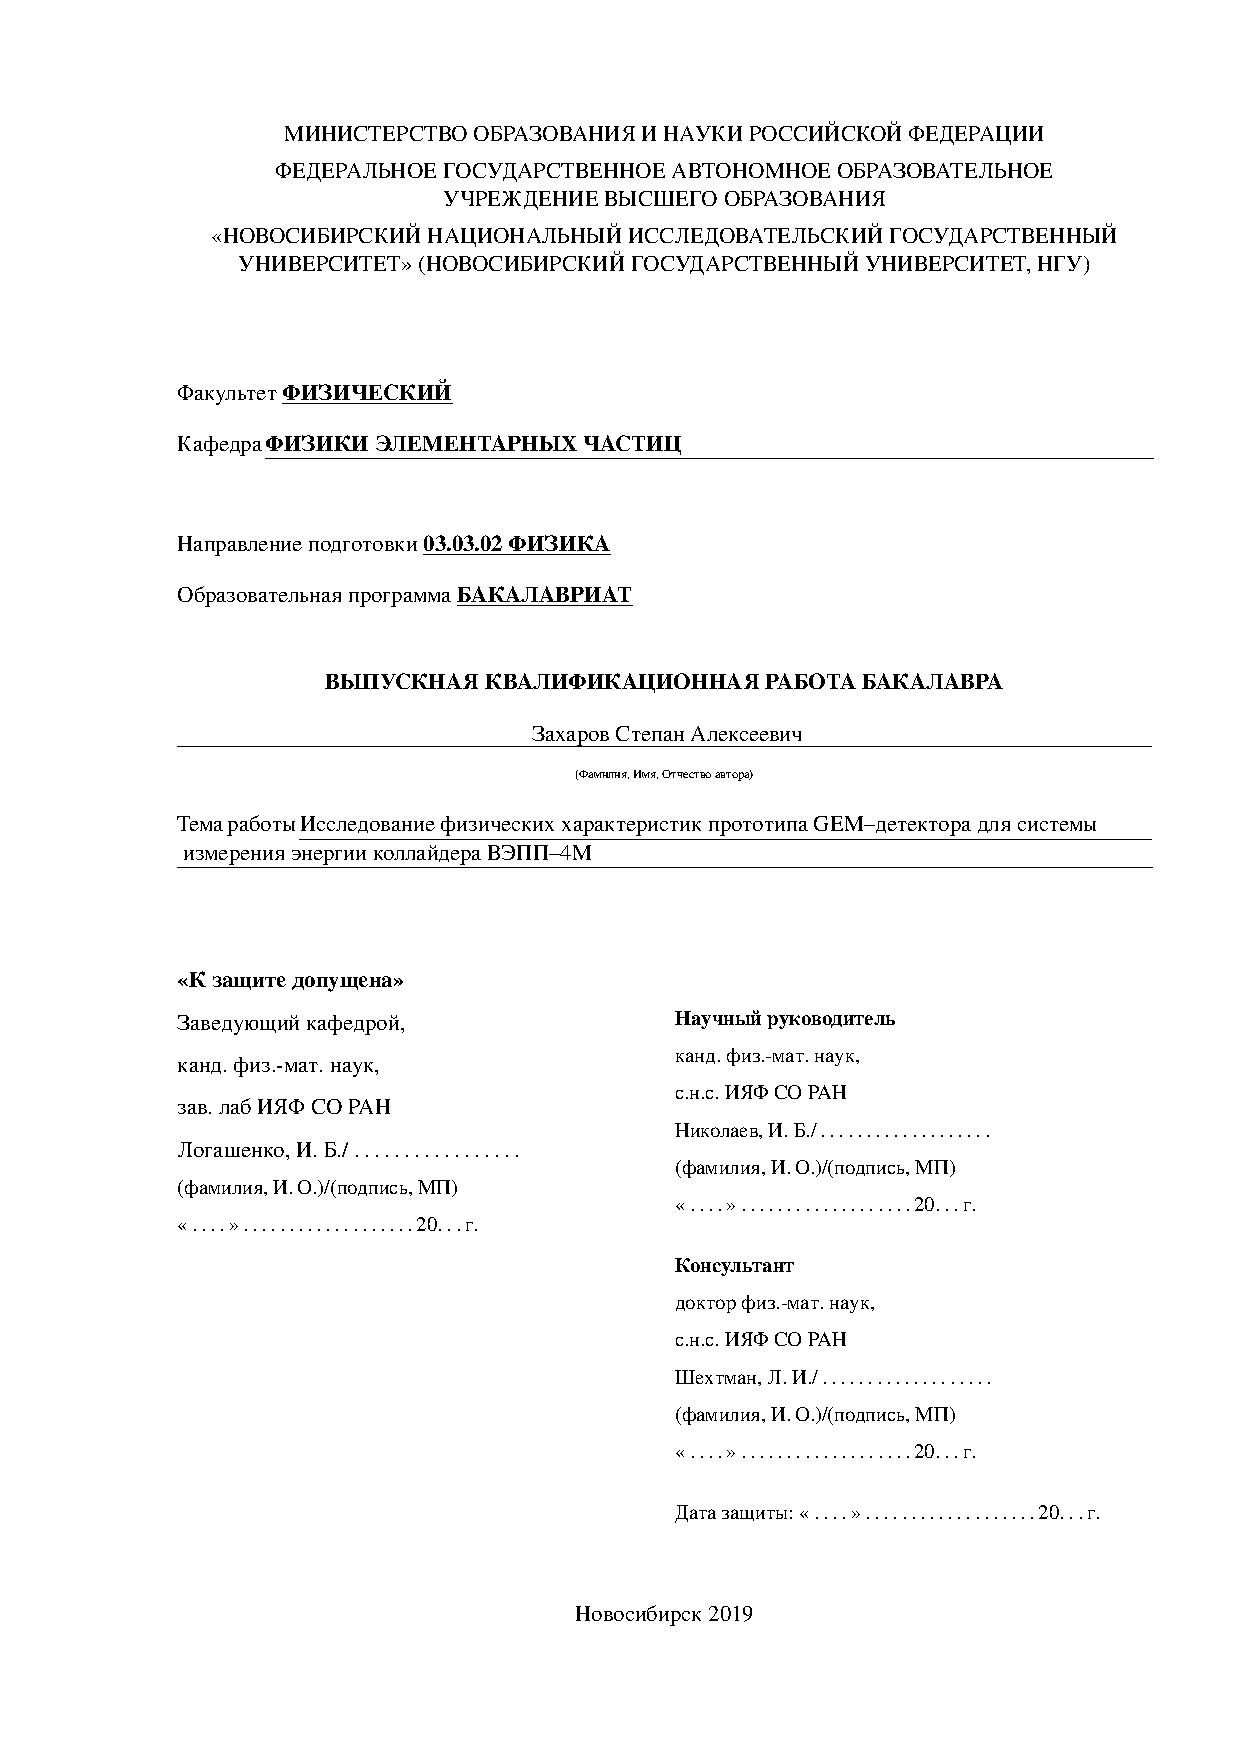
\includepdf{./titlepage/mytitle.pdf}
\newpage
\pagenumbering{goubble}
\tableofcontents
\newpage
\pagenumbering{arabic}
\setcounter{page}{4}
\pagestyle{plain}
\chapter*{Введение}
\label{sec:intro}
Развитие экспериментальных методов ядерной физики привело к появлению большого количества детектирующих систем. Отдельно стоит выделить координатные детекторы, по которым до сих пор ведутся активные исследования. Главными направлениями являются повышение эффективности регистрации и пространственного разрешения \cite{shechtman}.
\par Широкое распространение новых материалов и методов их обработки многократно улучшило параметры имеющихся детектирующих устройств, а так же позволило создавать детекторы новых конструкций. Так в 1997 г. группа ученых из Европейского центра ядерных исследований (CERN) под руководством Ф.~Саули успешно применила концепцию газового электронного умножения в микроструктурах для создания координатных детекторов, которые получили название <<GEM-детекторы>> или газовые электронные умножители \cite{sauli}. Их отличительными особенностями являются сравнительная простота конструкции, коэффициент усиления вплоть до $10^6$, а так же высокая радиационная стойкость. Данный тип детекторов широко используется в таких экспериментах, как PHOENIX (Франция), COMPASS (Швейцария), а так же в составе детекторов LHSb, TOTEM (ЦЕРН) и КЕДР (ИЯФ СО РАН).
\par В ИЯФ микроструктурные детекторы применяются не только в составе детекторов для экспериментов в ФЭЧ (КЕДР, СНД и КМД-3), но и в различных системах, связанных с ними. Одной из таких систем является установка <<лазерный поляриметр>>. В  основе её работы лежит предложенный в 1975 г. в ИЯФ метод резонансной поляризации \cite{bukin}. Применяется данная система для прецизионного измерения энергии на коллайдере ВЭПП-4М.
\par В рамках работ по усовершенствованию <<лазерного поляриметра>> планируется установить новый координатный детектор. Для выполнения данной задачи было решено использовать GEM-детекторы \cite{Bobr}. В ИЯФ существует возможность изготовления таких детекторов с использованием GEM-электродов, производимых в CERN. Таким образом, возникает необходимость в исследовании новых моделей GEM-детекторов.
\par \textbf{Целью данной работы} являлось создание и исследование характеристик GEM-детектора для установки <<лазерный поляриметр>>. Понимание физических процессов работы детектирующей системы, организацию модуля сбора данных, а также особенностей их анализа дает наиболее полную информацию о точности измерений.  
Для достижения поставленной цели были сформулированы основные задачи, которые определили ключевые направления деятельности:
\begin{itemize}
    
    \item Изучение физических основ работы газовых электронных умножителей и основных схем GEM-детекторов
    \item Определение основных параметров, влияющих на коэффициент усиления детектора 
    \item  Установка, настройка и управление механизацией детектора
    \item Создание и отладка системы сбора и обработки данных.
    \item Проведение экспериментов на выведенном пучке, в ходе которых исследованы физические характеристики детектора
    \item Обработка и анализ полученных данных 
	
\end{itemize}
\addcontentsline{toc}{chapter}{Введение}  
\newpage
\begingroup
	\let\clearpage\relax
	\chapter{Поляризационные эффекты и их применение для определения энергии пучка}
\label{sec:respnant_dep}
\section{Радиационная поляризация}
Эффект самопроизвольной поляризации заряженных частиц в ускорителях был описан Соколовым и Терновым еще в 1963г \cite{SokolovTernov63}. Качественно данный эффект можно описать следующим обоазом: в магнитном поле $\vec{H}$ потенциальная энергия частицы с магнитным моментом  $\vec{\mu}$ выражается как: 
\begin{equation}
U = - (\vec{\mu}, \vec{H}).
\end{equation} 
В случае поляризации пучка в ускорителе, $\boldsymbol{H}$ есть ведущее поле. Минимум потенциальной энергии дает значение угла между магнитным моментом и ведущим полем, равное нулю. Магнитный момент и спин электрона противоположно направлены, следовательно состояние электрона в пучке, в котором спин и магнитное поле антипараллельны, более устойчиво.
\par В работе  \cite{sokolov} определены доли от общего числа электронов, имеющие поляризацию против и по направлению поля: 
\begin{multicols}{2}
	\noindent
	\begin{equation}
	n_{\uparrow\downarrow} = \frac{15+8\sqrt{3}}{30} \approx 0.962 
	\end{equation}
	\begin{equation}
	n_{\uparrow\uparrow} = \frac{15-8\sqrt{3}}{30} \approx 0.038
	\end{equation}
\end{multicols}
Можно заметить, что практические все электроны в пучке имеют спин, направленный против ведущего поля. 
\section{Метод резонансной деполяризации}
Еще одним эффектом, возникающим при движении частиц со спином в электромагнитных полях, является прецессия спина $\vec{S}$ вокруг направления ведущего поля $\vec{H}$. Уравнение движения спина:
\begin{equation}
\cfrac{d\vec{S}}{dt} = [\vec{\Omega},\vec{S}],
\label{eq:precession_full}
\end{equation}
где $\vec{\Omega}$ имеет следующий вид:
\begin{equation}
\vec{\Omega} = -\biggl(\frac{q_0}{\gamma}+q'\biggr) \vec{H} + \frac{\gamma}{\gamma + 1}q' (\vec{\upsilon},\vec{H})\vec{\upsilon}- \biggl(\frac{q_0}{\gamma+1}  + q'\biggr)[\vec{\mathcal{E}},\vec{\upsilon}].
\end{equation}%
Здесь $q_0$ и $q'$ соответственно нормальная и аномальная части гиромагнитного отношения, $\gamma$ --- релятивистский гамма--фактор, $\vec{\upsilon}$ --- скорость частицы, $\vec{\mathcal{E}}$ --- вектор электрического поля.
В наиболее простом случае, когда $(\vec{\upsilon}, \vec{H})$ и $[\vec{\mathcal{E}},\vec{\upsilon}]$ равны нулю, имеем только один член, определяющий прецессию спина в ведущем магнитном поле. Таким образом, уравнение \ref{eq:precession_full} принимает вид:
\begin{equation}
\cfrac{d\vec{S}}{dt} = -\biggl(\frac{q_0}{\gamma}+q'\biggr) [\vec{H}, \vec{S}].
\label{eq:precession}
\end{equation}%
Если выразить ведущее поле через частоту обращения пучков как: 
\begin{equation}
\vec{H} = \frac {\gamma mc}{e}\omega_r\vec{n}_H.
\label{eq:larmor_freq}
\end{equation}
Подставим \ref{eq:larmor_freq} в \ref{eq:precession} и проведем серию математических преобразований чтобы получить выражение для частоты прецессии спина:
\begin{equation}
\omega_s=  \omega_{r}\bigg(\frac{q'}{q_0}\frac{E}{mc^2}+1\bigg).
\label{eq:spin_freq}
\end{equation}
Если измерить $\omega_s$ и $\omega_{r}$, то можно определить энергию электрона $E$ т.к. остальные константы в выражении \ref{eq:spin_freq} известны. $\omega_{r}$ можно найти разными способами: прямым измерением с помощью pickup--станций, по частоте ускоряющего поля в резонаторе и т.д. Однако, определение $\omega_s$ является весьма нетривиальной задачей. 
\par Один из методов, с помощью которого можно косвенно измерить  $\omega_s$ по регистрации резонансной деполяризации предварительно поляризованного пучка частиц, был разработан в ИЯФ СО РАН в 1974 г. и детально описывается в \cite{skrinskii}. Идея метода заключается в воздействии на пучок переменного электромагнитного поля определенной частоты. Если выполняется резонансное условие:
\begin{equation}
\omega_s=  k\omega_{r} \pm \omega_d,
\end{equation}
где $\omega_d$ -- частота электромагнитного поля, то исходная поляризация пучка нарушается. Это можно определить любым поляризационно чувствительным методом. Проводя сканирование по $\omega_d$ и фиксируя момент деполяризации, можно определить $\omega_s$.
\par Приведем оценку точности данного метода. Для этого определим какова точность определения параметров, входящих в выражение \ref{eq:spin_freq}:
\begin{itemize}
	\item $\displaystyle \frac{\delta (q'/q_0)}{q'/q_0} = 2.24 \cdot 10^{-10} $ \cite{PDG}
	\item $\displaystyle \frac{\delta (mc^2)}{mc^2}= 6.06\cdot10^{-9} $ \cite{PDG}
	\item $\displaystyle \frac{\delta (\omega_r)}{\omega_r} = 10^{-12} ~???$
\end{itemize}
Можно заметить, что точность определения массы электрона вносит наибольший вклад в точность измерения энергии. Физическое ограничение для $\delta E/E$ устанавливается на уровне $10^{-8}$. Измерения, использующие метод резонансной деполяризации, являются на данный момент самыми точными в мире.
\section{Регистрация эффекта деполяризации}
Существует несколько методов, с помощью которых можно зарегистрировать момент деполяризации. Все они предполагают рассеяние электронов пучка на ядрах --- Моттовское рассеяние, на электронах этого же пучка --- Тушековское рассеяние, а также Комптоновское рассеяние на поляризованных фотонах. Первый метод малоэффективен ввиду отсутствия в вакуумной камере достаточного количества атомов, на которых рассеивался бы пучок. Установки, использующие эффект Тушековского или внутрисгусткового рассеяния широко используются на малых энергиях ($E < 2~\GeV$). Из-за того, что измеряемый эффект обратно пропорционален четвертой степени энергии пучка, то в области $\Upsilon$---резонанса его применение является малоэффективным.
\par В данном случае Комптоновское рассеяние поляризованных фотонов на пучке электронов является единственным методом, применимым в данном диапазоне энергий. Сечение рассеяния зависит как от поляризации электрона, так и от поляризации фотона. Идея метода заключается в следующем: если пучок электронов поляризован, то существует связь между направлением рассеяния фотонов и их поляризацией. Изменяя направление поляризации (используя например левоциркулярные и правоциркулярные лазерные пучки), можно регистрировать рассеяние преимущественно в верхнюю или нижнюю полуплоскость т.к. поляризация электронов вертикальная, а значит в системе существует выделенное направление. В таком случае величина измеряемого эффекта определяется формулой:
\begin{equation}
	\Delta y = \frac{\hbar \omega_0}{2 m_e c^2} \mathcal{P} \Delta V L,
\end{equation}
где $\omega_0$ -- частота падающего фотона, $\mathcal{P}$ -- поляризация электронного пучка, $\Delta V$ -- разница стоксовских параметров для циркулярно поляризованного пучка фотонов, $L$ -- расстояние от точки взаимодействия до точки регистрации рассеянного фотона. При деполяризации электронного пучка $\mathcal{P} = 0$, следовательно вертикальная асимметрия рассеяния фотонов пропадает. Чтобы это зарегистрировать, необходим координатный детектор с достаточным разрешением. В нём эффект деполяризации будет выглядеть как слияние двух отдельных пятен, расположенных друг над другом, в одно пятно. 


	\vspace{24pt}
\chapter{Координатные детекторы на основе GEM}
\label{sec:coor_GEM}
\section{Общие принципы работы газовых координатных детекторов}
Измерения координат частиц проводятся с помощью довольно широкого спектра устройств, использующих различные физические принципы в основе своей работы. В отдельную группу стоит выделить газовые координатные детекторы. В основу их работы легло явление ионизации атомов газа первичной заряженной частицей. Если зарегистрировать первичную ионизацию -- заряд, образовавшийся после пролета частицы через чувствительную область детектора, то можно восстановить её координаты. Основная проблема заключается в том, что для первичной частицы ионизация составляет по порядку величины $10 \div 100$ электрон--ионных пар на 1 см трека. Регистрация таких малых зарядов представляется проблематичной. Поэтому в детекторной технике используются различные усиливающие устройства, которые позволяют увеличивать количество заряда до значений, при которых его можно зарегистрировать современными зарядочувствительными устройствами \cite{grupen}.
\par При создании детектора для установки <<Лазерный поляриметр>> были выдвинуты требования, которые позволили определить тип используемой усилительной системы и общую схему детектора. Наиболее важные из них: 
\begin{itemize}
	\item регистрация координат фотонов
	\item достаточное для достоверного наблюдения эффекта порядка 0.1\,мм пространственное разрешение 
	\item возможность одновременного детектирования нескольких фотонов
	\item компактные размеры, простота и надежность конструкции
\end{itemize}
Регистрация фотонов с энергиями $\sim1\GeV$ обычно производится посредством их конверсии в электрон--позитронные пары и последующей регистрации уже заряженных частиц. После рассмотрения возможных схем, удовлетворяющих данным требованиям, было решено остановиться на т.н. микроструктурных детекторах, как на наиболее простых и, в то же время, обеспечивающих требуемое пространственное разрешение. Это достаточно новый тип детекторов \cite{sauli}, однако в ИЯФ СО РАН накоплен сравнительно большой опыт по работе с ними.
\section{Газовые микроструктурные детекторы}
Идея использования микроструктурных газовых координатных детекторов получила развитие в CERN в 1980--х г. Многие детекторы данного типа имеют схожий принцип работы: с помощью проводников определенной формы в газовой среде создаются локальные области с высокой напряженностью поля. При попадании в них, заряженная частица на длине свободного пробега приобретает энергию, большую, чем энергия ионизации атомов газовой смеси. 
\begin{figure}[h]
	\centering
	\begin{subfigure}{.45\textwidth}
		\centering
		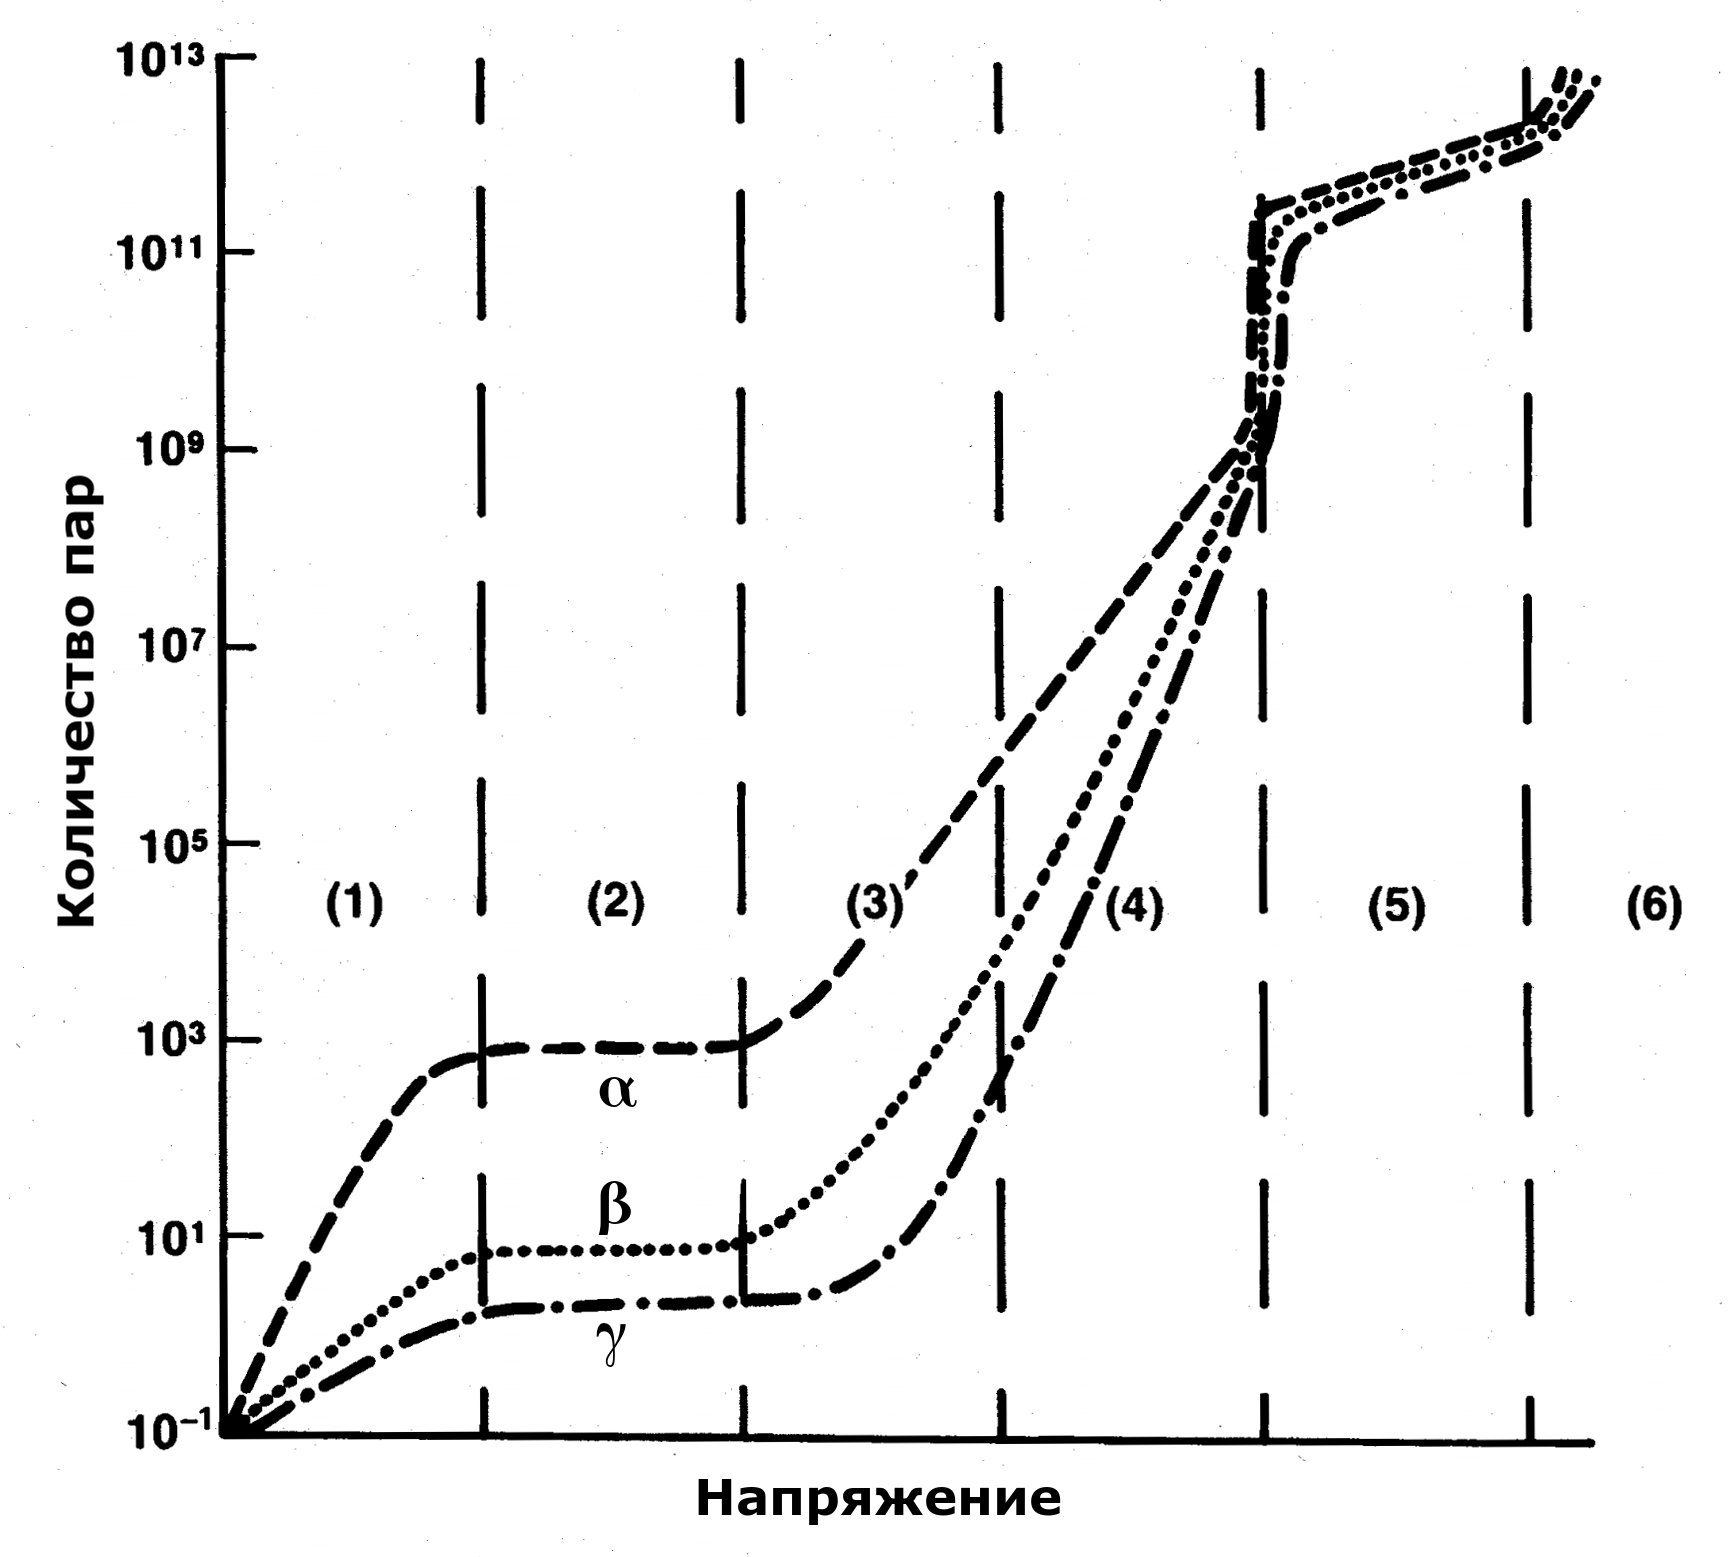
\includegraphics[width=0.9\linewidth]{img/Gas_discharge_gr.png}
		\caption{Зависимость удельного количества электрон-ионных пар от напряжения, приложенного электродам в газовом промежутке. Количество ионизации различно для $\alpha,\beta$ и $\gamma$--частиц.}
	\end{subfigure}
	\hspace{20pt}
	\begin{subfigure}{.45\textwidth}
		\centering
		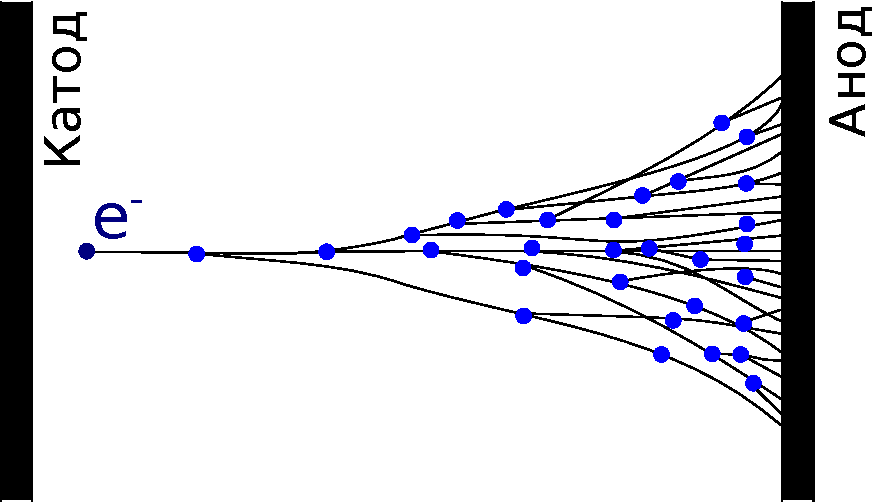
\includegraphics[width=1\linewidth]{img/Electron_avalanche.pdf}
		\caption{Образование электронной лавины. В пропорциональном режиме количество вторичных электронов экспоненциально растет с координатой, вдоль которой движется частица. Полное их число пропорционально первичной ионизации}
	\end{subfigure}%
	\caption{Режимы работы газовых детекторов определяются напряженностью электрического поля в газовом промежутке, которое зависит от напряжения на электродах детектора и его геометрии. Микроструктурные детекторы работают в пропорциональной области (3)}
	\label{fig:gas_discharge}
\end{figure}
 Поэтому становится возможным образование электрон-ионных пар. Из-за того, что подвижность ионов почти на 3 порядка меньше подвижности электронов, основной вклад в эффект объясняется движением электронов. Более того, количество заряженных частиц экспоненциально растет, но электрического пробоя не происходит. Это объясняется определенной геометрией электродов, а так же экранировкой внешнего поля полем свободных зарядов. Т.к. микроструктурные детекторы работают в пропорциональном режиме, то суммарное количество заряда пропорционально первичной ионизации.
 \par Рассмотрим подробнее один из видов микроструктурных детекторов -- газовые электронные умножители, которые было решено применены в конструкции  Они были впервые созданы группой Ф. Саули в CERN в 1997 г. и на данный момент активно исследуются и применяются в современных детектирующих системах. 
 \begin{figure}[h]
 	\centering
 	\begin{minipage}{.45\textwidth}
 	\centering
 	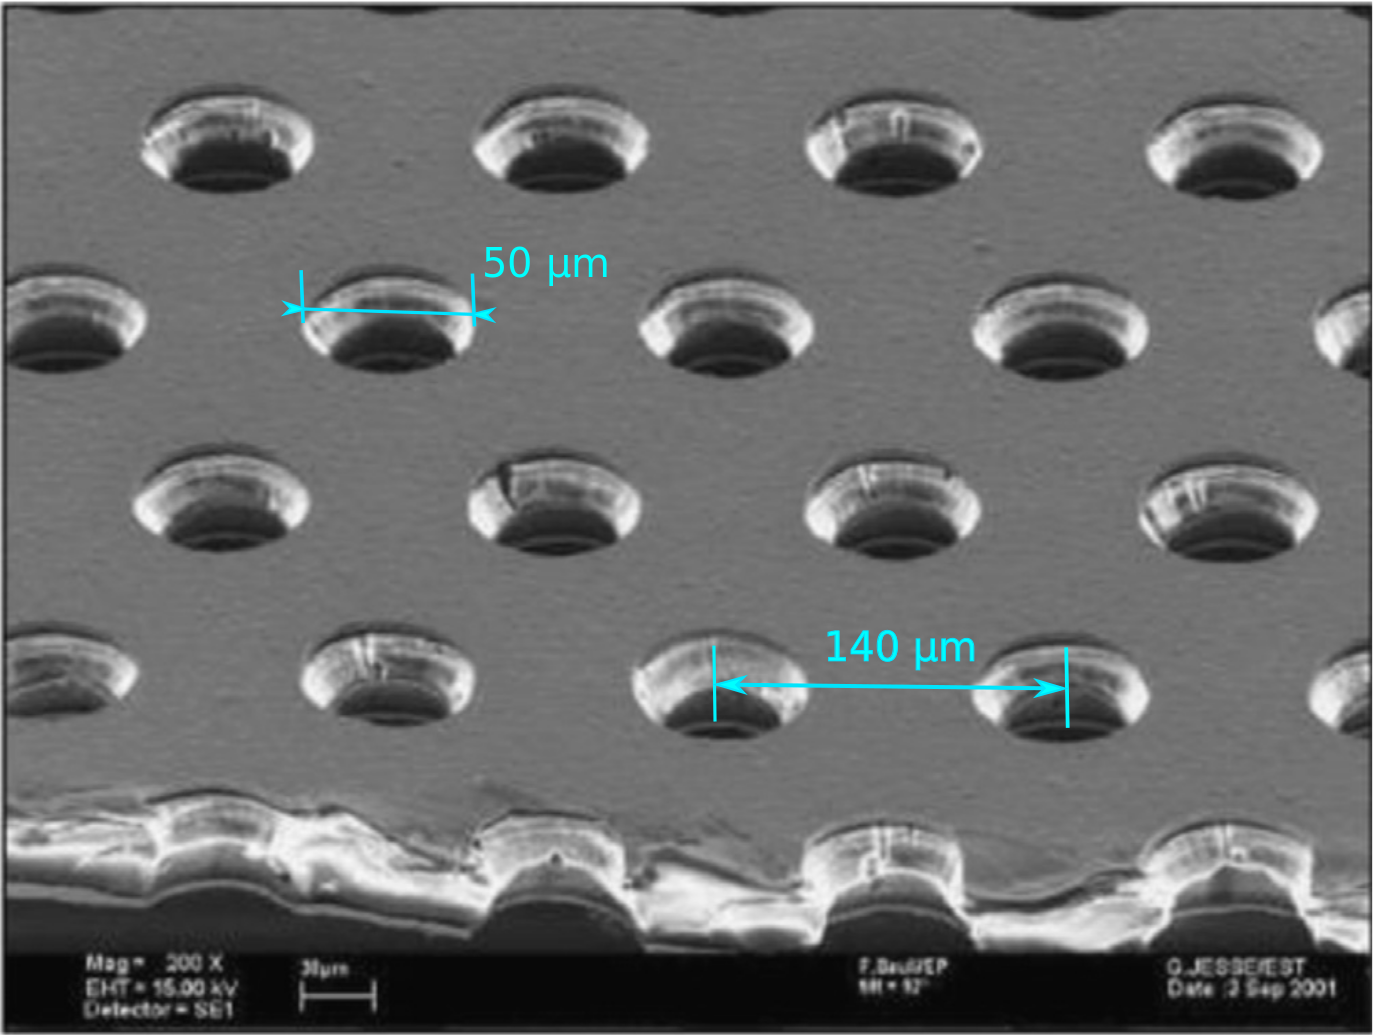
\includegraphics[width=1\linewidth]{img/GEM_microphoto.png}
 	\caption{Микрофотография GEM. Видны последовательные ряды отверстий конической формы, протравленных в медном электроде и полиимидной пленке.}
 	\end{minipage}
 	\hspace{20pt}
 	\begin{minipage}{.45\textwidth}
 			\centering
 		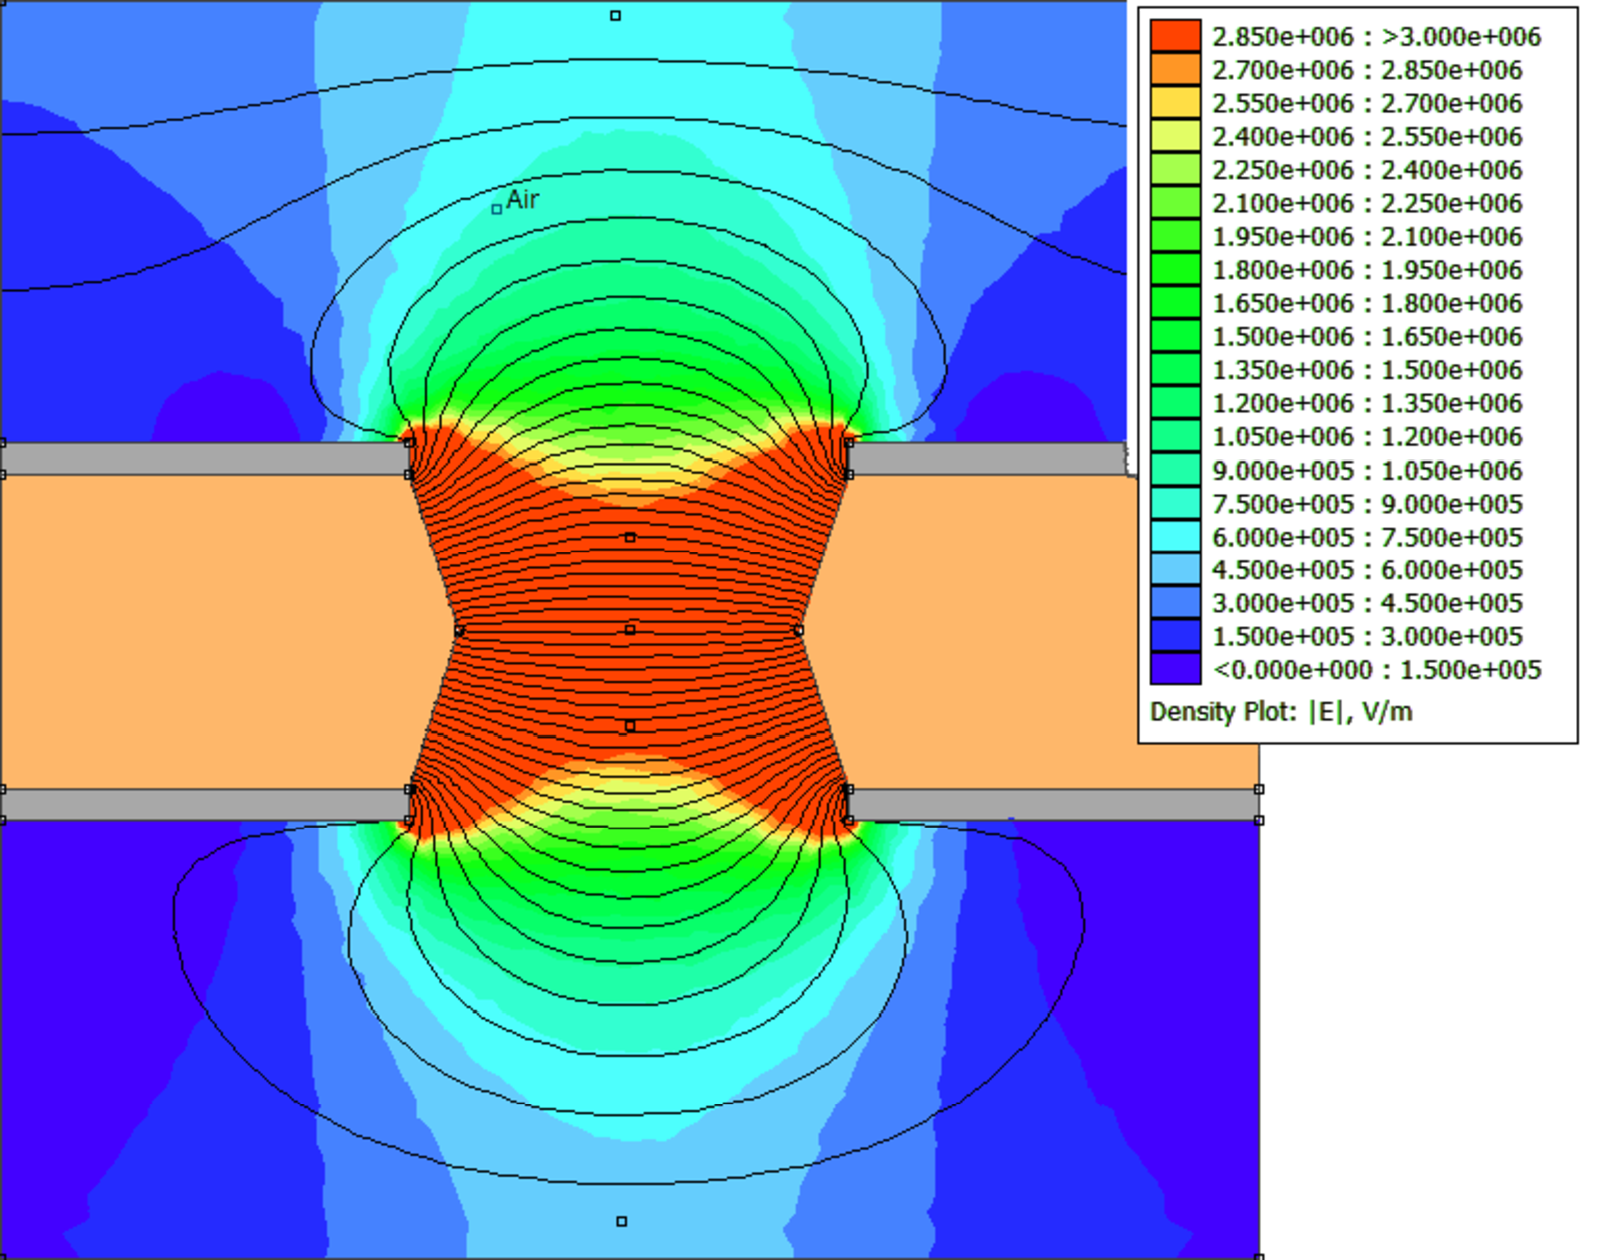
\includegraphics[width=1\linewidth]{img/GEM_field.pdf}
 		\caption{Моделирование распределения электрического поля в отверстии GEM методом конечных элементов.}
 	\end{minipage}
 \end{figure}
 Газовый электронный умножитель представляет собой полиимидную плёнку толщиной 50\,мкм, покрытую с двух сторон слоями меди, толщиной 5\,мкм. В слоях меди и полиимида протравливаются отверстия размером 50\,мкм с шагом 140\,мкм. Такая конструкция позволяет точно (до 100\,нм) выдерживать размеры отверстий и расстояние между электродами, а значит и величину электрического поля в отверстиях. Этот параметр напрямую влияет на коэффициент усиления и прозрачность GEM, а в конечном итоге на эффективность регистрации и надежность детектора.
 \par Наиболее простая конструкция детектора на основе  GEM состоит из катодного электрода, в качестве которого обычно применяют фольгированный полимид, анодного электрода (или группы электродов в случае координатного детектора) и GEM, расположенного между ними.
 \begin{figure}[h]
	\centering
	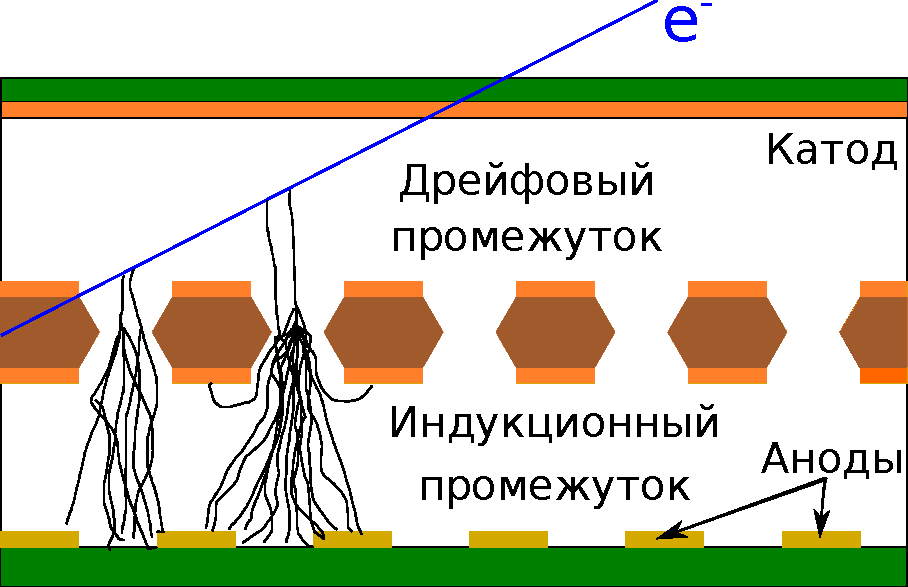
\includegraphics[height = 4 cm, width= 6cm]{img/GEM_scheme.pdf}
	\caption{Схема детектора на основе GEM. Первичная частица вызывает ионизацию в дрейфовом промежутке, которая, проходя через GEM--электрод создает электронные лавины, регистрируемые считывающей структурой.}
	\label{fig:single} 	
 \end{figure}
  следующий: к медным электродом прикладывается напряжение порядка 300 В, и в отверстиях создается поле порядка 1 МВ/м. Первичная ионизирующая частица проникает в дрейфовый промежуток, где ионизирует атомы газовой смеси. Электроны ионизации дрейфуют к GEM--электроду, в котором образуются электронные лавины. Вторичная ионизация попадает в индукционный промежуток и регистрируется анодами детектора.
 \par В случае когда требуется обеспечить большие коэффициенты усиления или высокую эффективность регистрации, электроды GEM можно размещать последовательно, формируя дополнительные транспортные промежутки. Так можно достичь коэффициентов усиления вплоть до $10^7$ \cite{sauli}. Ограничением на максимальное количество заряда, образуемое в электронной лавине, то есть на максимальный коэффициент усиления является т.н. предел Рейтера, который равняется приблизительно $Q_{max} = 10^6\div10^7~e^-$. При достижении зарядом лавины данного значения вероятность электрического пробоя резко возрастает, поэтому следует выбирать оптимум по параметрам детектора между усилением схемы и вероятностью возникновения пробоя. 
  
 




	\chapter{Исследование прототипа детектора для установки <<Лазерный поляриметр>>}
\label{sec:pol_examine}
\section{Конструкция детектора}
Для регистрации одиночных гамма--квантов, полученных обратным комптоновским рассеянием на пучках электронов, был спроектирован и изготовлен прототип детектора, использующего ГЭУ для усиления сигнала первичной ионизации. В конструкции применен тройной электрод с питанием от резистивного делителя. Основа детектора представляет собой многослойную плату из СТЭФ с массивом плоских металлических электродов, расположенных в её центральной части, которую можно видеть на Рис. \ref{fig:Detector_full_fig} 
\begin{figure}[H]
	\centering
	\begin{subfigure}{.5\textwidth}
		\centering
		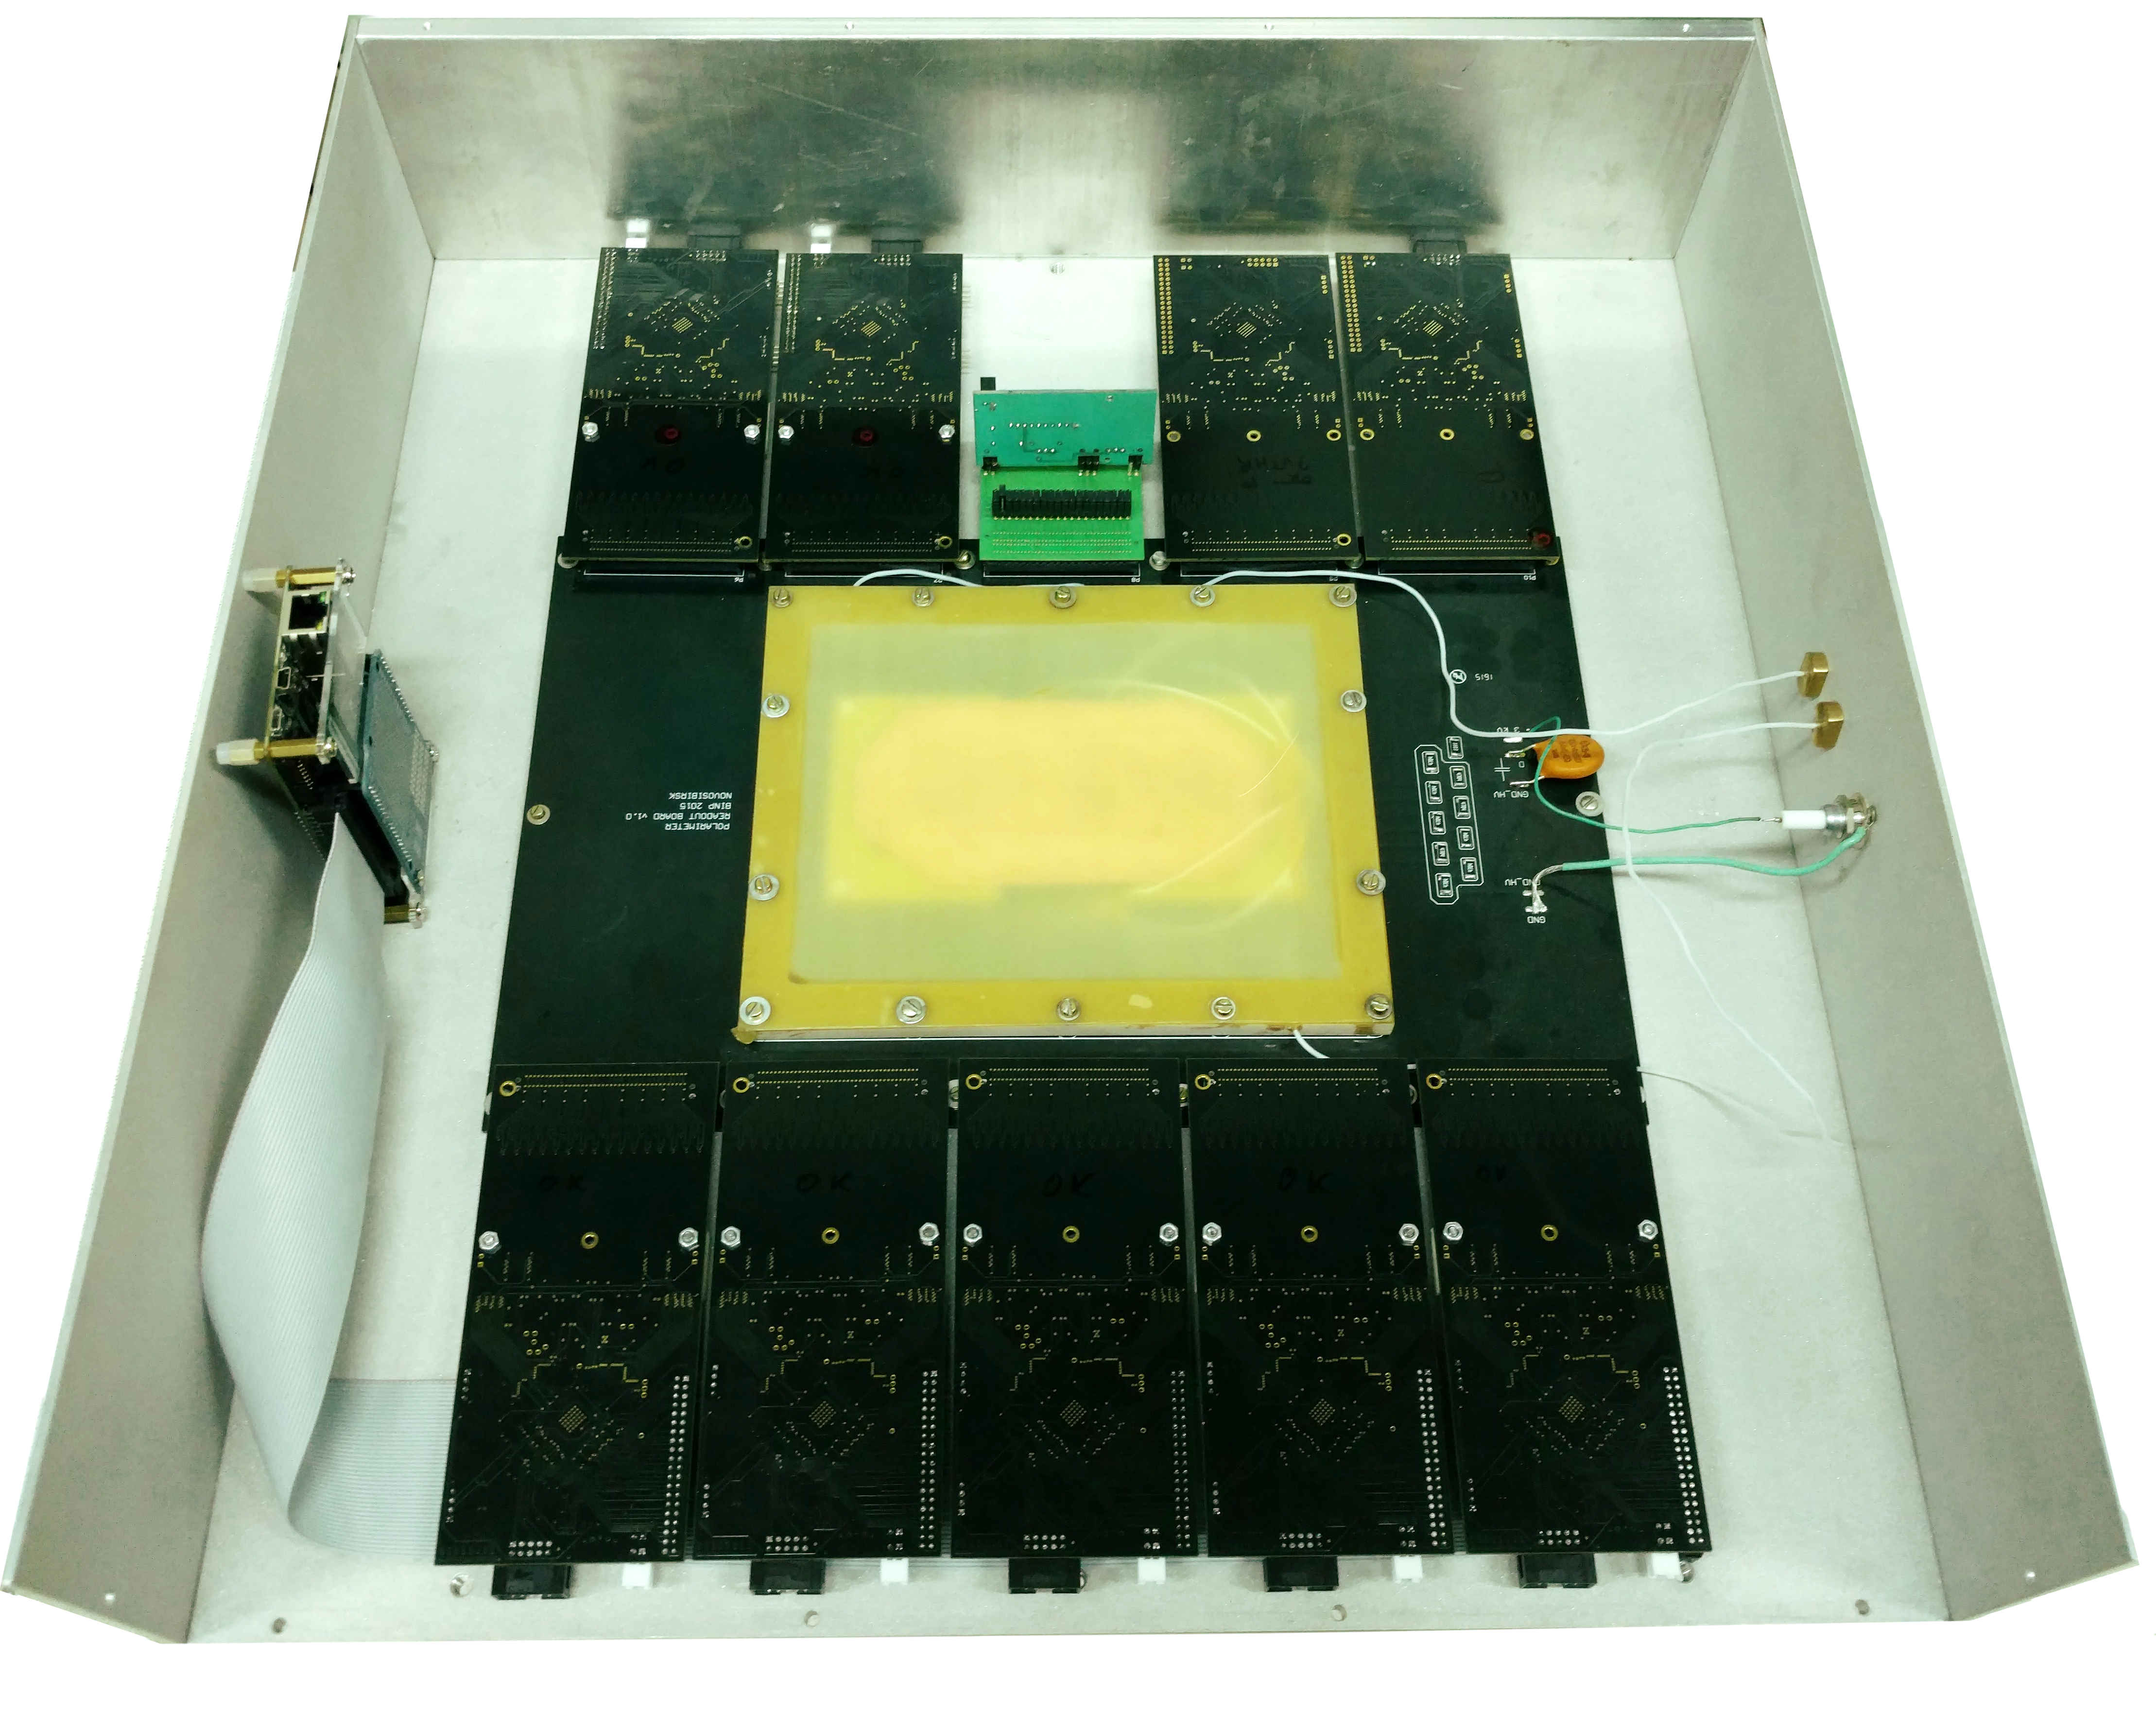
\includegraphics[height = 5 cm, width= 5.5cm]{img/GEM_prototype.jpg}
		\caption{Детектор в сборе}
		\label{fig:Detector}
	\end{subfigure}%
	\begin{subfigure}{.5\textwidth}
		\centering
		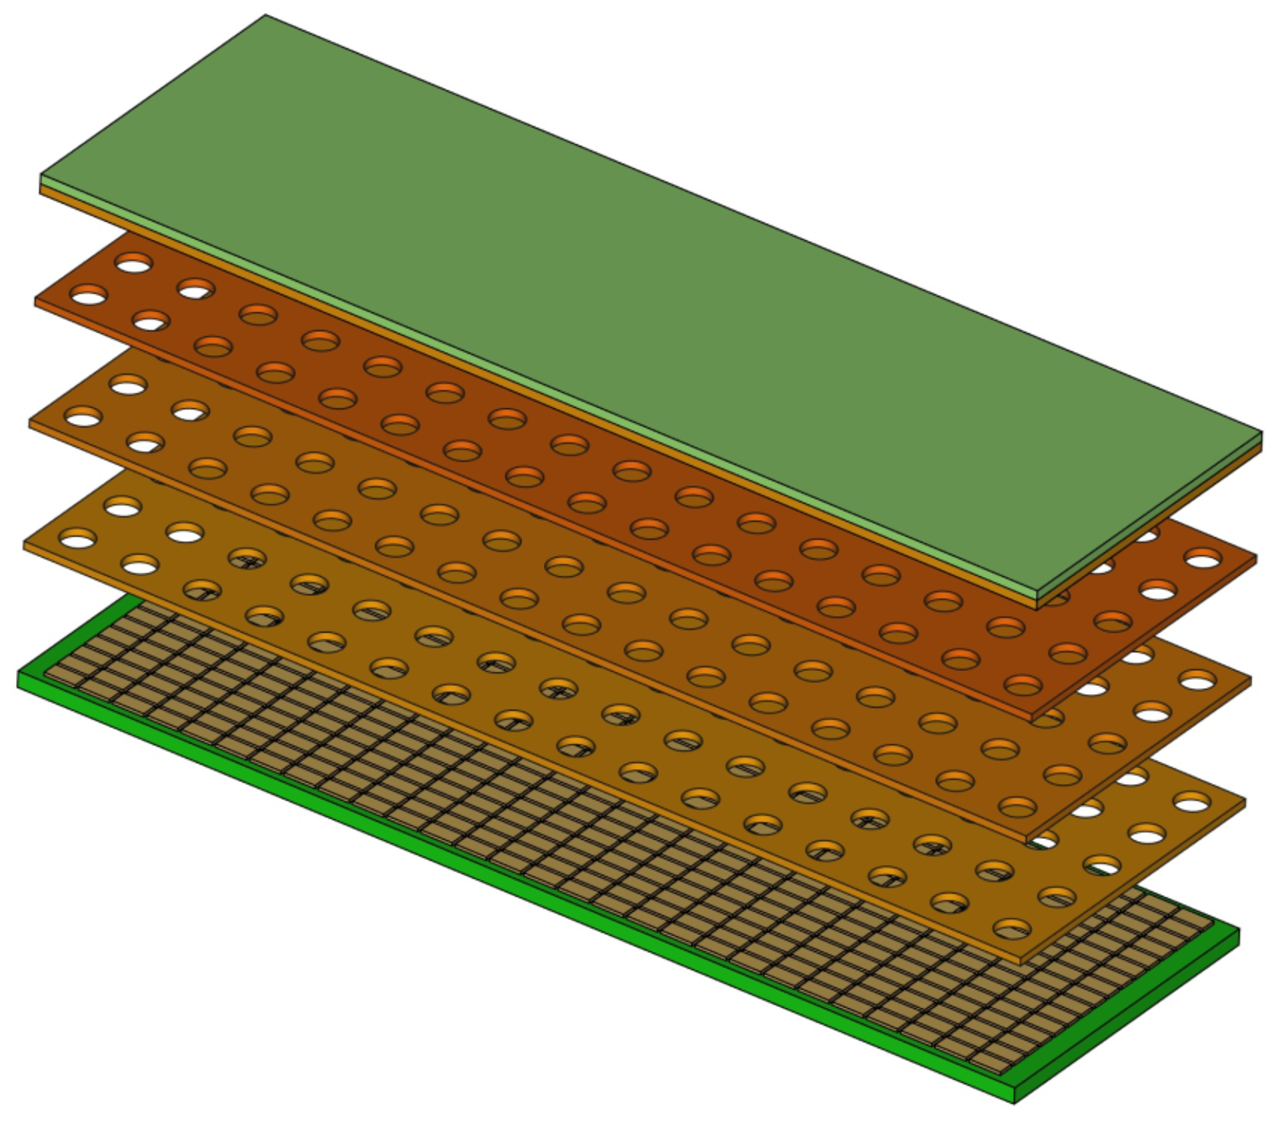
\includegraphics[height = 5 cm, width= 5.8cm]{img/GEM_model.pdf}
		\caption{Схема ускоряющей структуры}
		\label{fig:GEM_structure}
	\end{subfigure}
	\caption{Прототип дететкора для <<Лазерного поляриметра>>. Он включает главную плату с ускоряющей структурой из трех GEM -- электродов и считывающую структуру, а также разъемы для подключения десяти front--end плат.}
	\label{fig:Detector_full_fig}
\end{figure}
\par Электроды ГЭУ укреплены на рамках из 1.5 мм СТЭФ над считывающей структурой. Сверху на плату закрепляется герметичный кожух из СТЭФ с трубками для ввода и вывода газовой смеси. Сборка детектора осуществляется в корпусе из листового алюминия.
\par Данный детектор отличается от аналогов типом считывающей структуры (Рис. \ref{fig:readout_structure}), которая позволяет регистрировать события с высокой множественностью. Это является критическим параметром для <<Лазерного поляриметра>> ввиду того, что за одну вспышку лазера по расчетам на пучке будет происходить рассеяние порядка 10 фотонов. Возможность регистрации каждого из них существенно увеличит статистику и, тем самым, повысит точность измерения энергии.
\begin{figure}[H]
	\begin{center}
		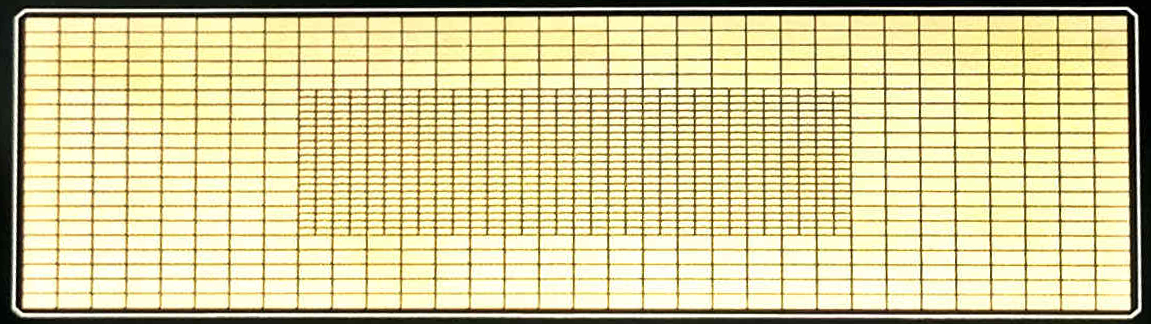
\includegraphics[width = 10cm]{img/Main_board_pads.jpg}
		\caption{Считывающая структура детектора выполнена в виде отдельных прямоугольных металлических площадок. В центральной области размер площадки $1\times2$ мм, в периферийной области --- $2\times4$ мм. Всего на плате 1120 каналов}
		\label{fig:readout_structure}
	\end{center}%
\end{figure}%
\noindent Заряд с электродов считывается  посредством десяти front-end плат. Они установлены в специальные многоканальные разъемы на периферии основной платы. Front-end электроника включает в себя быстрые АЦП и ПЛИС для работы с ними. Далее сигнал по USB подается на компьютер. На данный момент разрабатывается программное обеспечивающее взаимодействие всех 10 плат и одновременное считывание события с детектора. Решено было использовать для последующих экспериментов только одну из плат, т.к. вычитывание данных с неё уже отлажено. 
\section{Особенности сбора и обработки сырых данных}
\label{sec:DAQ_raw_data}
Каналы детектора объединены в группы по 100 (центральная часть) или 120 (периферия) каналов. Каждая группа скоммутирована на отдельный разъем, к которому подключены два многоканальных АЦП. Одновременно можно вычитывать данные со всех каналов. При поступлении сигнала с триггера, схема начинает последовательно раз в 125 нс вычитывать заряд со всех каналов. Таким образом вычитывание происходит 100 раз. Каждый отсчет времени будем в дальнейшем называть <<кадром>>, а массив данных о заряде для каждого из каналов группы и каждого кадра из 100 назовем <<событием>>. 
\par Из-за технических особенностей схемы нулевой уровень сигнала составляет 7400 каналов АЦП. Сигнал, соответствующий пришедшей на электрод ионизации, представляет собой импульс отрицательной полярности, который имеет резкий передний фронт (1 кадр) и экспоненциально затухающий задний фронт (3-10 кадров в зависимости от суммарного заряда). Для последующей обработки сигнала, из него необходимо вычесть пьедестал. С этой целью в программе управления считывающей платой реализована возможность получения усредненных данных о пьедесталах, которые затем записываются в отдельный файл формата TXT. На Рис. \ref{pedestal_map} представлены гистограммы для пьедесталов одной считывающей платы.
\begin{figure}[H]
\begin{center}
	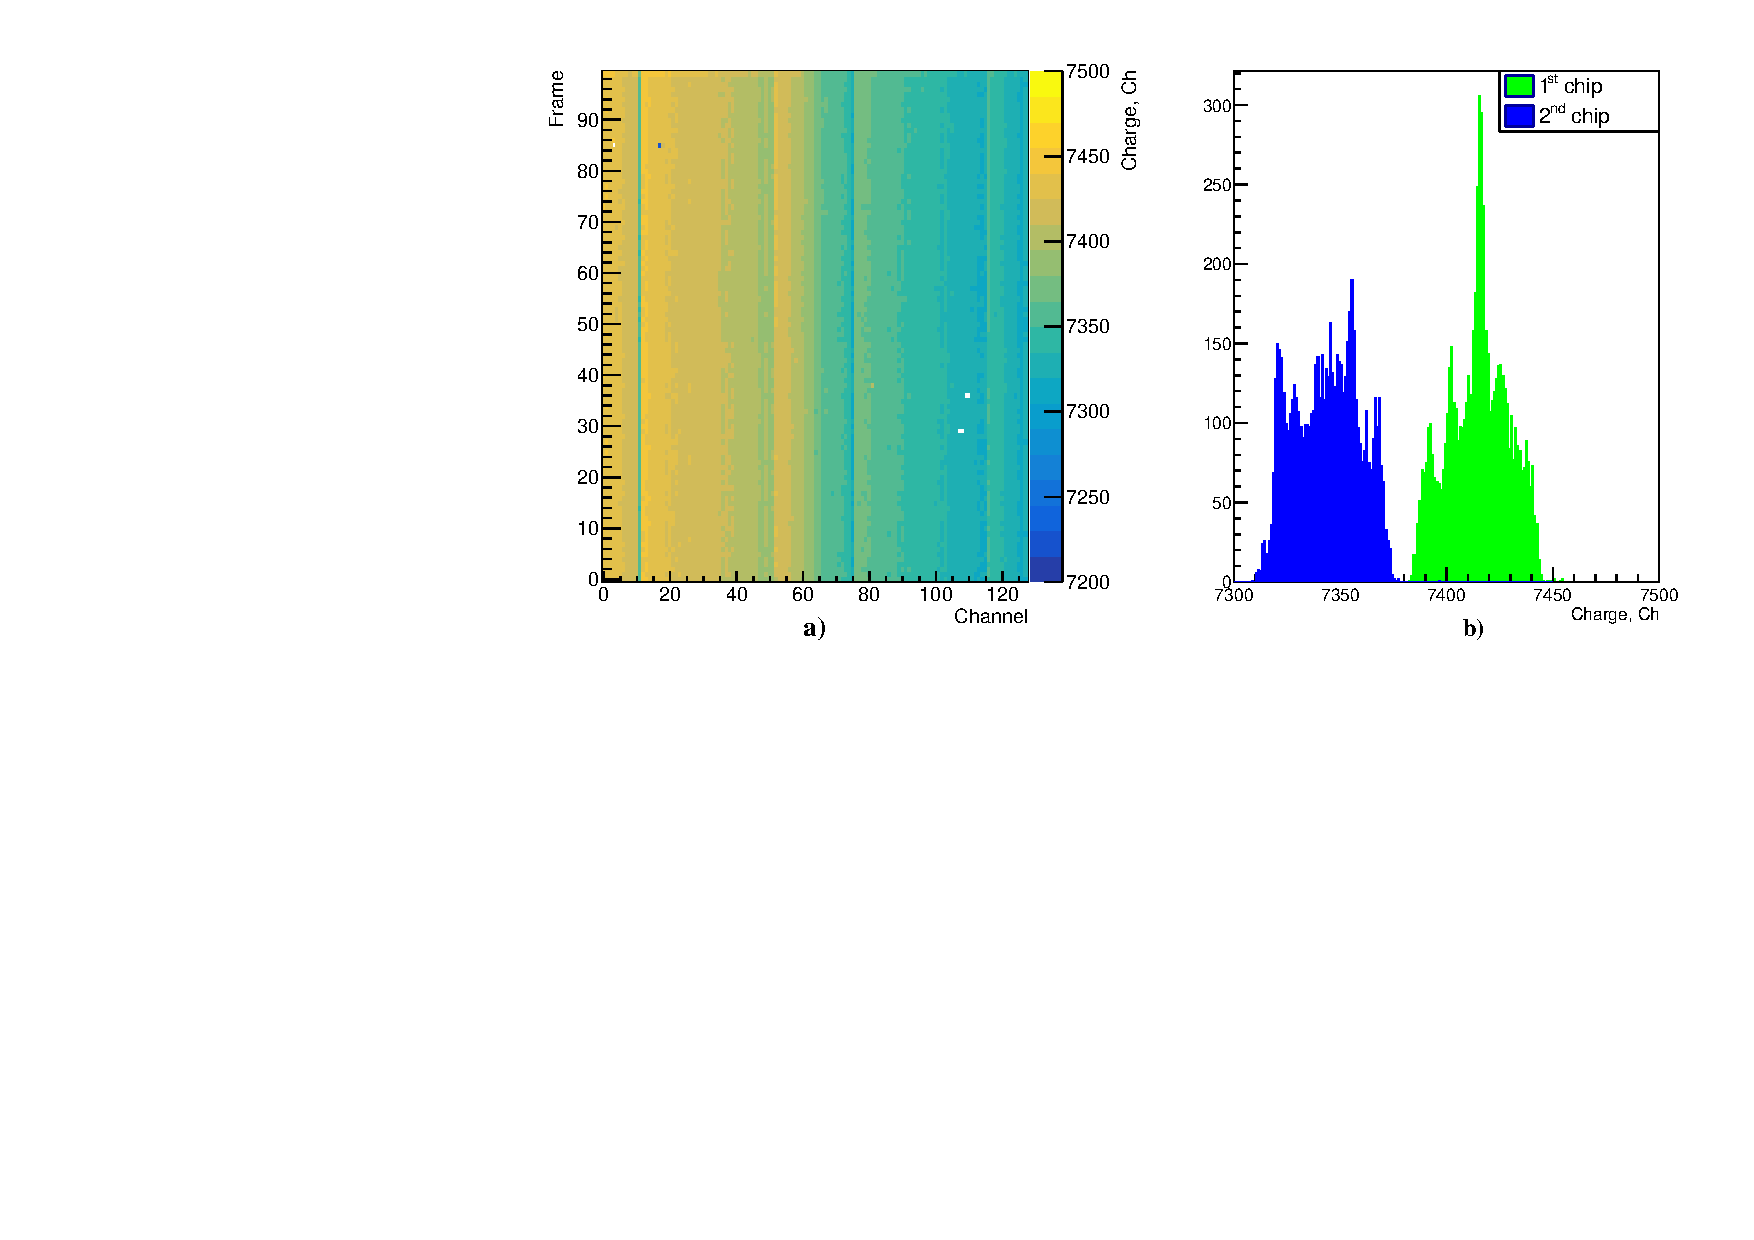
\includegraphics[width = 12cm]{img/pedestal_map.pdf}
	\caption{a): Карта пьедесталов АЦП. По горизонтальной оси обозначены номера каналов одной группы (Channel). По вертикальной оси --- кадры (Frame). Значения заряда показаны на цветовой шкале и лежат в пределах 7200--7500 каналов АЦП (Ch). b): Распределение заряда по каналам для первого и второго чипа считывающей платы}
	\label{pedestal_map}
\end{center}
\end{figure}
Можно заметить, что существует как разброс значений пьедестала в одном чипе, так и между чипами в плате. Поэтому решено было вычитать из сигнала пьедестал, соответствующий данному каналу.
\par События последовательно записываются в TXT--файл. Формат вывода следующий: строка соответствует одному кадру и состоит из 128 чисел. Всего таких строк в событии 100. 101--я строка содержит номер кадра, с которого началось вычитывание значений АЦП. Данная информация важна по следующей причине: микросхемы АЦП непрерывно вычитывают заряд с каналов, но ПЛИС возвращает событие только при активации триггера. Это сделано для того, чтобы исключить накопление заряда на входах АЦП и искажения данных о сигнале. Ввиду возможного разброса параметров электронных компонентов внутреннего pipeline АЦП, необходимо определять пьедесталы не только для каждого канала, но и для каждого кадра в канале. Поэтому номер канала в последней строке события дает необходимую привязку к физическим кадрам АЦП и позволяет правильно вычитать пьедесталы.
\par В ходе работы с прототипом детектора было обнаружено, что некоторые каналы имеют на порядок больший уровень шума, поэтому решено было их значения занулять и в анализе не использовать. 


\section{Обработка сигнальных событий}
Электронная лавина обычно регистрируется не одним каналом считывающей структуры, а несколькими. Это вызвано диффузией носителей в газовых промежутках детектора, что вызывает увеличение поперечных размеров области с носителями. Назовем такое распределение заряда от одной электронной лавины кластером. На мониторе события, который представлен на Рис. \ref{event_map}, можно видеть группы вертикальных желтых полос. Это и есть кластеры. Заряд в них экспоненциально убывает со временем. Для анализа же требуется только значение с первого кадра, где наблюдается превышение уровня заряда над фоном.   
\begin{figure}[H]
	\begin{center}
		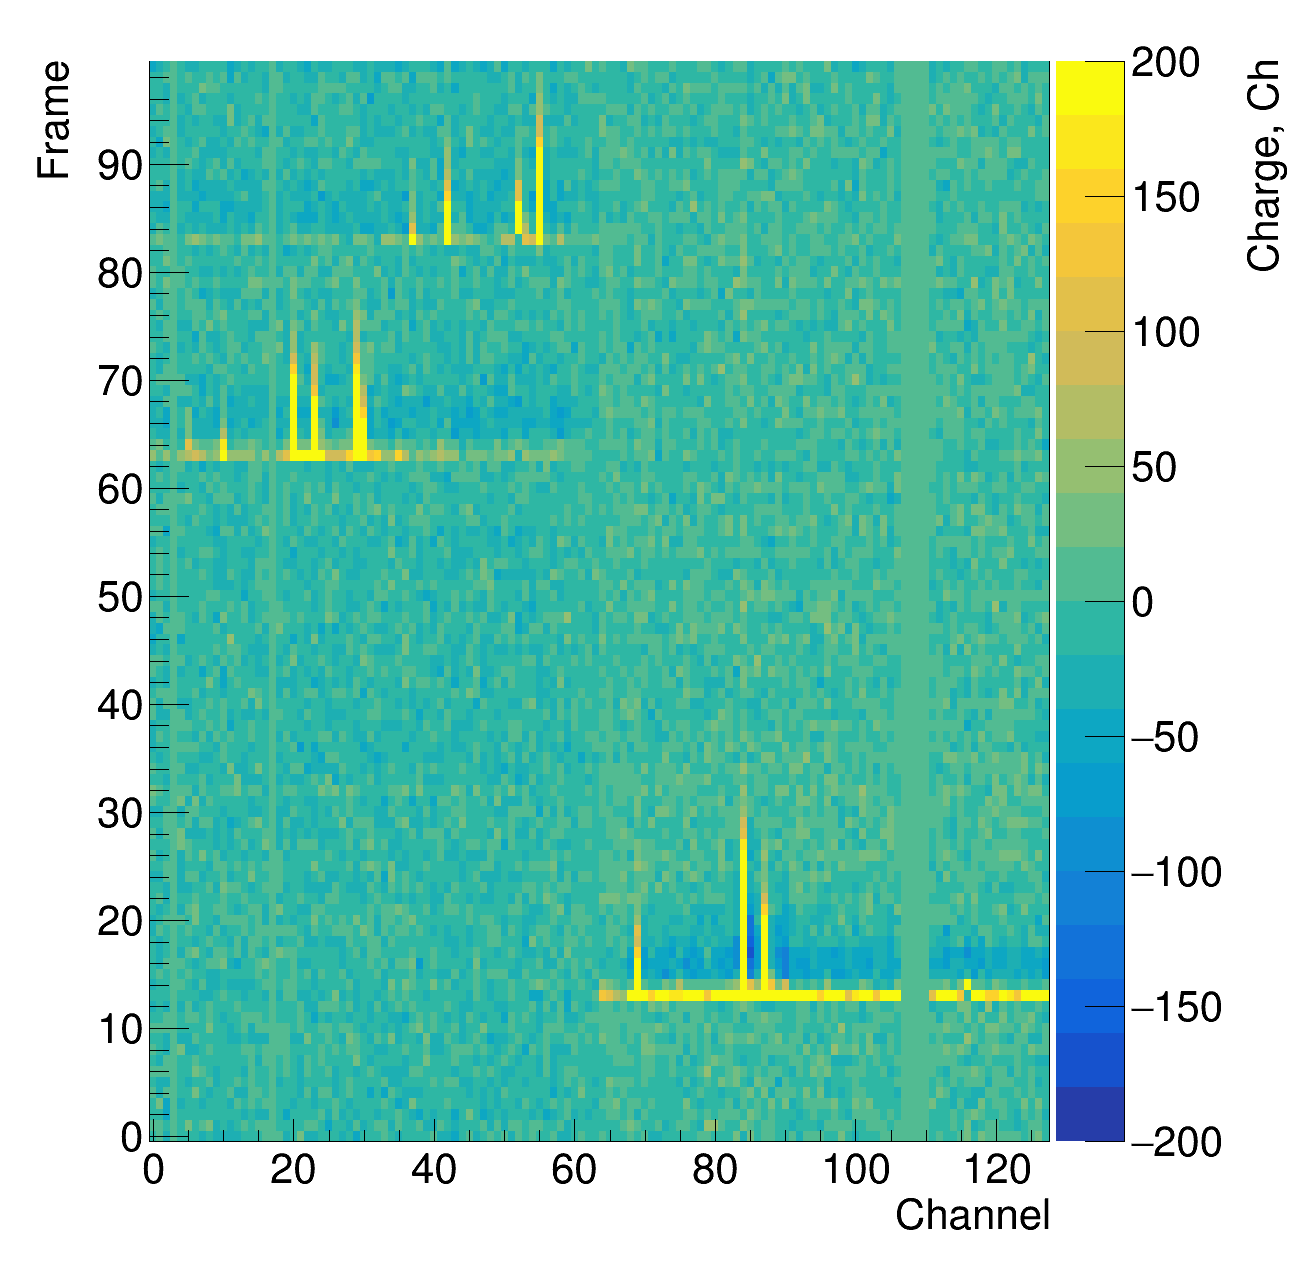
\includegraphics[width = 8cm, height = 7cm]{img/Signal.png}
		\caption{Вид сигнального события. Регистрировались $2.2~\MeV$ электроны источника $Sr-90$. По вертикальной оси отложены кадры, по горизонтальной - канале. Цвет показывает значение заряда в конкретном канале и кадре. В данном событии зафиксировано три кластера (два в первом чипе и один во втором)}
		\label{event_map}
	\end{center}
\end{figure}%
 Заряд кластера является ключевой характеристикой при определении коэффициента усиления детектора. Поэтому необходим алгоритм, который ассоциирует группу каналов с кластером и вычисляет его заряд. С этой целью для детектора <<Лазерного поляриметра>> на языке Python написана библиотека, осуществляющая обработку первичных данных с детектора. В ней реализованы следующие алгоритмы:
 \begin{itemize}
 	\item предобработка данных события:
 	\begin{itemize}[label=$\circ$]
 		\item чтение файлов <<сырых данных>>
 		\item вычитание пьедесталов
 		\item маскировка шумовых каналов
 	\end{itemize}
 	\item фильтрация сигнальных событий
 	\item привязка номера канала АЦП к координатам считывающей площадки на плате
 	\item нахождение кластера и определение его заряда
 \end{itemize}
Особенности предобработки данных обсуждались выше (см. п. \ref{sec:DAQ_raw_data}). Рассмотрим работу остальных алгоритмов.
\subsection{Привязка каналов к их физическим координатам}
Чтобы привязать канал АЦП к координатам считывающей площадки, необходимо знать карту каналов. Она была получена путём прямого измерения и сверена со схемой считывающей платы. Необходимость измерения в первую очередь была продиктована высокой плотностью расположения электродов на плате, а так же необходимостью проверки работоспособности её электрических соединений. 
\begin{figure}[H]
	\centering
	\begin{subfigure}{.5\textwidth}
		\centering
		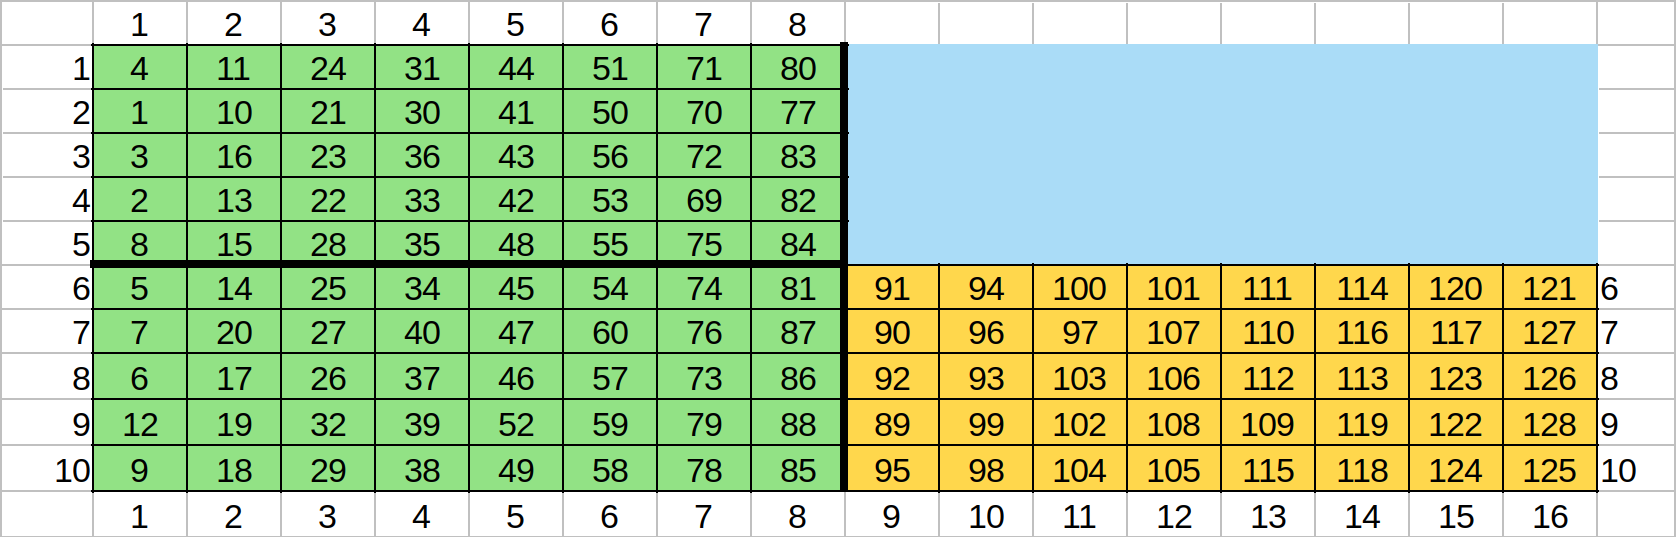
\includegraphics[height = 2.5cm]{img/Side_pixmap.png}
		\caption{Периферийная часть}
	\end{subfigure}%
	\begin{subfigure}{.5\textwidth}
		\centering
		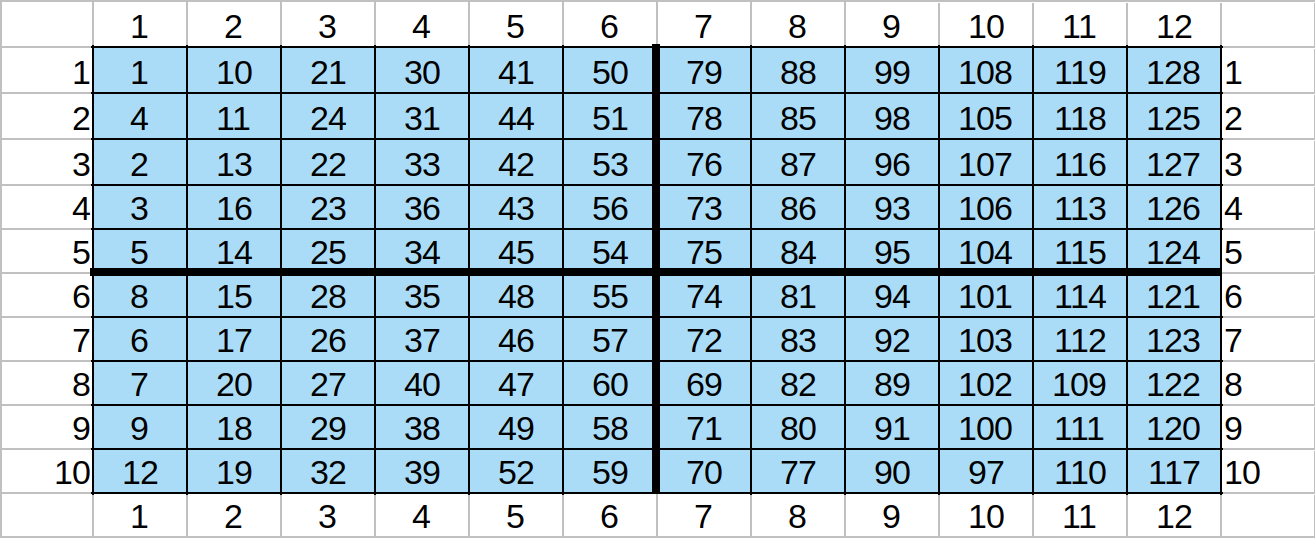
\includegraphics[height=2.5cm]{img/Center_pixmap.png}
		\caption{Центральная часть}
	\end{subfigure}
	\caption{Карты расположения считывающих площадок и номера каналов, которые им соответствуют. Представлено два случая расположения: для платы из периферийной и центральной областей. В цветных клетках указан номер канала АЦП, соответствующий данной считывающей площадке. Цифры вокруг цветной области - координаты считывающих площадок.}
	\label{fig:pixmap}
\end{figure}
Возьмем для примера центральную область. Считанное из файла событие преобразуется во временный двумерный массив ($128\times100$), а затем в соответствии с картой каналов данные из него перегружаются в трехмерный массив ($12\times10\times100$), первые две координаты массива соответствуют координатам считывающей структуры. Восемь каналов: $60\div67$ не используются, и входы АЦП, соответствующие им, не подключены к считывающей структуре. Дальнейшая работа проводится с этим трехмерным массивом.
\subsection{Коррекция нулевого уровня в кадрах}
\par Первичные эксперименты с детектором показали, что при регистрации кластера с большим значением заряда нулевой уровень шумовых каналов смещается. Результат этого виден на Рис. \ref{event_map}, где средний уровень кадра находится в желтой области, что говорит о его смещении на 100-200 каналов. Т.к. при регистрации кластера этот систематический сдвиг будет смещать значение каждого канала, то суммарная ошибка определения заряда кластера возрастёт в $\sqrt{N_{Ch}}$ раз, где $N_{Ch}$ -- количество сработавших каналов. Поэтому необходимо каким-то образом произвести поправку на систематический сдвиг нулевого уровня заряда для каждого кадра.
\begin{figure}[H]
	\centering
	\begin{subfigure}{.33\textwidth}
		\centering
		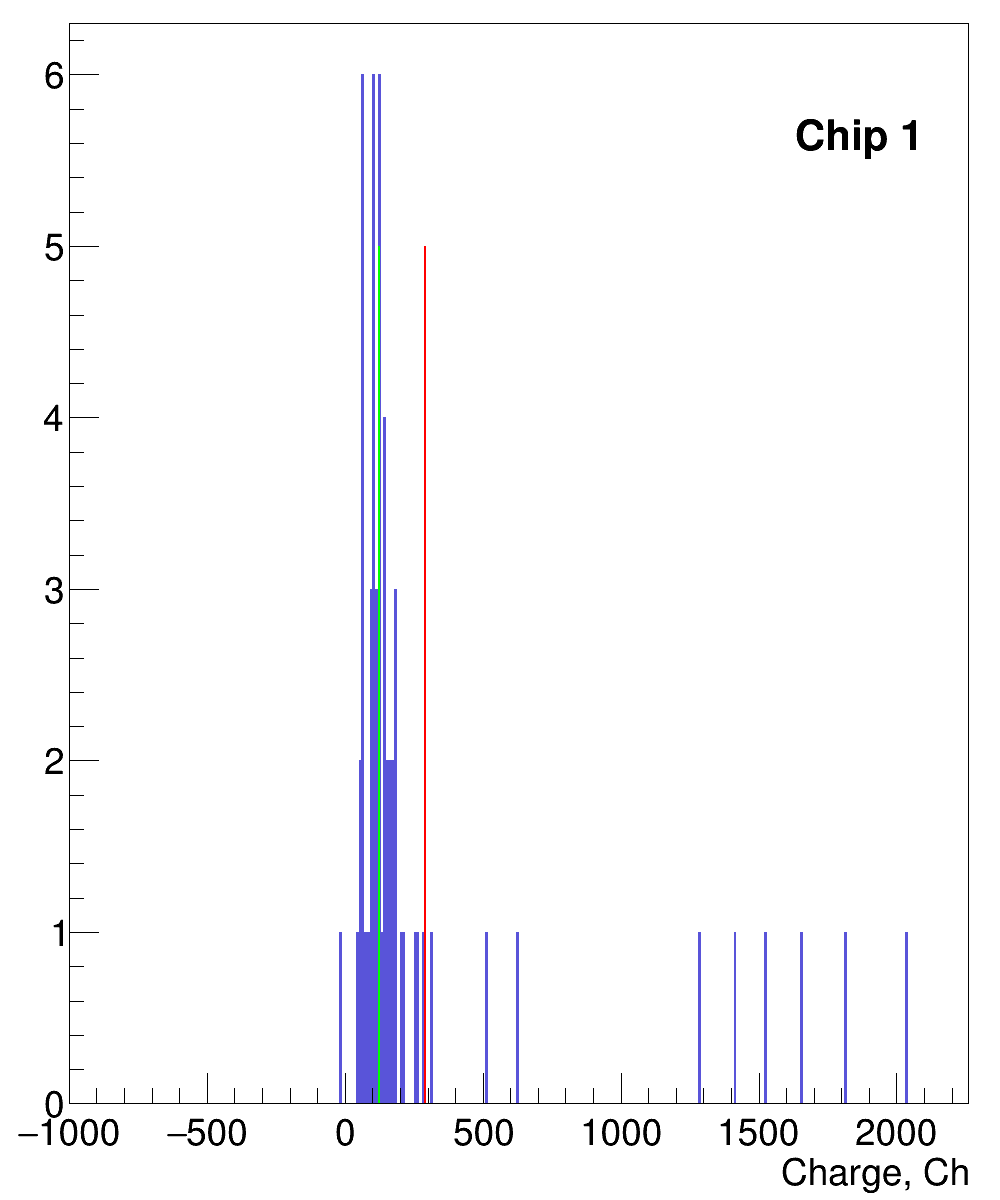
\includegraphics[height = 6.5 cm, width= 5.5cm]{img/Median_unzoomed.png}
		\caption{Распределение заряда\\в кадре}
		\label{fig:median_signal}
	\end{subfigure}%
	\begin{subfigure}{.33\textwidth}
		\centering
		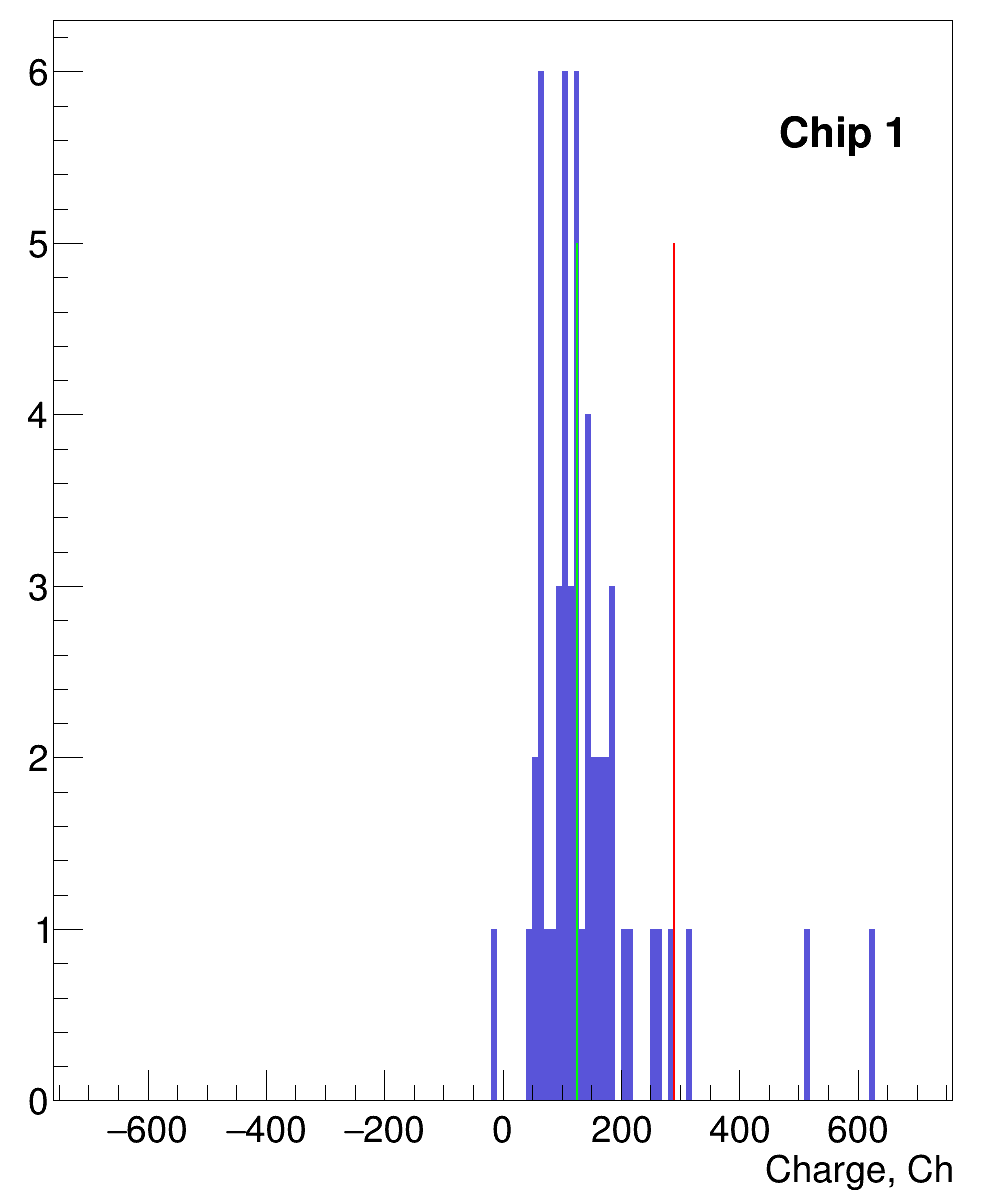
\includegraphics[height = 6.5 cm, width= 5.8cm]{img/Median_1.png}
		\caption{Шумовые каналы \\ (без~фильтра)}
		\label{fig:median_noize}
	\end{subfigure}
	\begin{subfigure}{.33\textwidth}
		\centering
		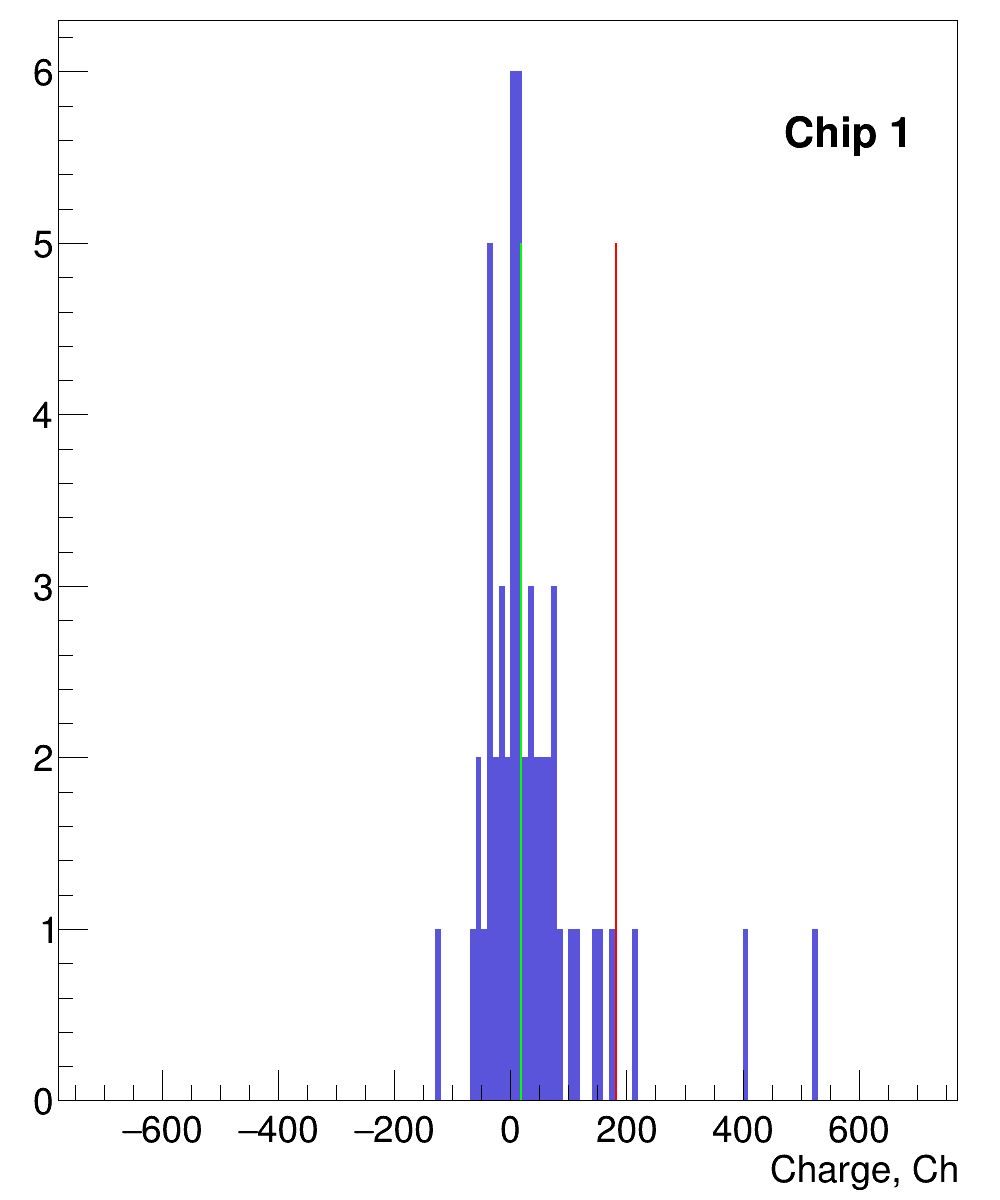
\includegraphics[height = 6.5 cm, width= 5.8cm]{img/Median_0.png}
		\caption{Шумовые каналы\\(с~фильтром)}
		\label{fig:medianF_noize_biased}
	\end{subfigure}%
	\caption{Распределение заряда в сигнальном кадре. Красная вертикальная линия показывает среднее значение по распределению. Зеленая -- медиану распределения. Медиана дает более точную оценку среднего по шумам, что позволяет сделать поправку и сместить средний уровень кадра к нулю.}
	\label{fig:medianF}
\end{figure}
Если построить распределение по заряду в каналах одного кадра, то можно заметить, значения заряда шумовых каналов  сгруппированы вблизи нуля, а заряд от сигнальных каналов находится далеко справа от нуля (Рис. \ref{fig:median_signal}.) Более того, на Рис. \ref{fig:median_noize} виден сдвиг среднего значения шумов относительно нуля. Можно заметить, что использование обычного порогового фильтра в данном случае малоэффективно по двум причинам:
\begin{enumerate}
	\item Систематический сдвиг нулевого значения канала может стать причиной ошибочного распознавания шумовых каналов, как сигнальных
	\item При малом заряде кластера сигнальные каналы могут быть приняты за шумовые
\end{enumerate}
 Перед нами возник вопрос: как определять пороговое значение для разделения сигнала и шума? Для решения этой задачи была реализована идея медианного алгоритма, графическое представление которой можно видеть на Рис.\ref{fig:medianF}. 
 \par Суть алгоритма заключается в вычислении медианы распределения по заряду для отдельного кадра. Причем при небольшом количестве сработавших каналов медиана достаточно точно описывает среднее значение заряда по шумовым каналам, которое, после вычитывания пьедесталов, должно равняться нулю. Если сдвинуть значение заряда в каждом канале кроме канала с максимальным зарядом на вычисленную медиану, то это позволяет подавить систематический сдвиг нулевого уровня в кадре. 
 \subsection{Поиск кластеров и определение их заряда}
 Алгоритмическая часть, отвечающая за регистрацию кластеров на данный момент активно разрабатывается. Поэтому система имеет ограниченный функционал: регистрирует только один кластер в событии. 
 \begin{figure}[h]
 	\begin{center}
 		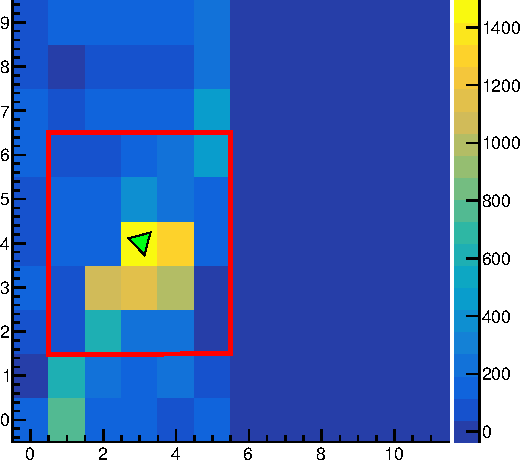
\includegraphics[width = 6cm, height = 4.5cm]{img/cluster_padmap.pdf}
 		\caption{Сигнальное событие. По вертикали и горизонтали отложены условные координаты считывающих площадок. Цвет соответствует заряду в конкретном канале. Площадка с максимальным зарядом помечена зеленым треугольником, вокруг неё имеются каналы желтого цвета -- кластер. Окрестность, из которой будет производиться вычитывание заряда, отмечена красным квадратом}
 		\label{fig:cluster_padmap}
 	\end{center}
 \end{figure}
 Это происходит в два этапа: сначала определяется канал и кадр с максимальным значением заряда после этого генерируется окрестность в виде квадрата размером $5\times5$ считывающих площадок, по которым происходит суммирование значений заряда, если в конкретном канале его значение превышает шум. Последняя величина была дополнительно определена как уровень шумов -- параметр $\sigma$ из аппроксимации гауссовой функцией распределения по заряду шумовых каналов, умноженный на масштабный коэффициент (в данном случае 5), которым можно регулировать избирательность алгоритма. Подробнее о шумах можно узнать из пункта \ref{sec:noise_study}
 
 
 

	\vspace{24pt}
\chapter{Исследование физических характеристик детектора <<Лазерного поляриметра>>}
\section{Определение уровня шумов детектора}
\label{sec:noise_study}
\begin{figure}[H]
	\begin{center}
		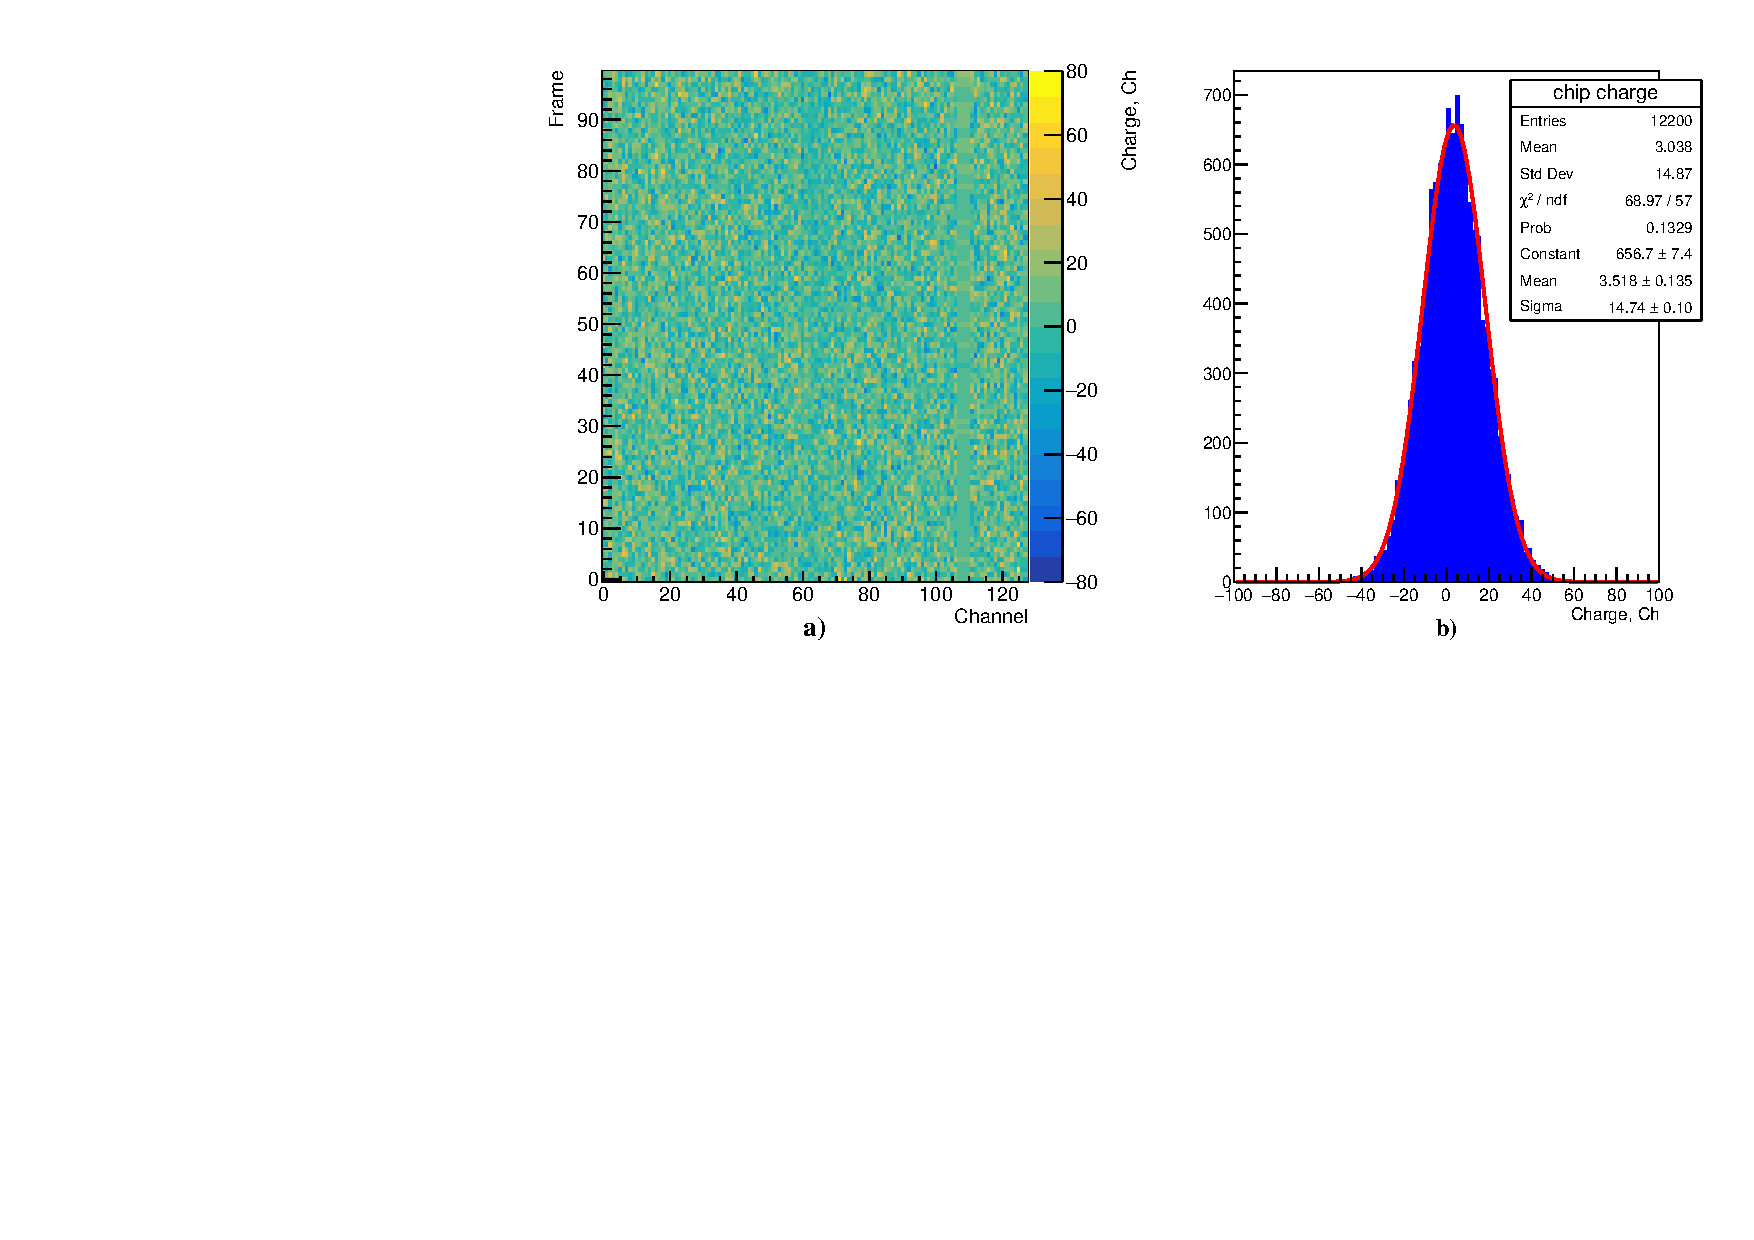
\includegraphics[width = 12cm, height = 6cm]{img/noise_map.pdf}
		\caption{a): Вид шумового события после вычитания пьедестала b): Распределение заряда в шумовом событии}
		\label{noise_map}
	\end{center}
\end{figure}
Рис. \ref{noise_map} показывает вид одного шумового события и распределение заряда в кадрах и каналах. Важным значением, которое можно извлечь уже из одного шумового события является уровень шумов. Его можно определить как корень из дисперсии распределения на Рис. \ref{noise_map} b). Шумы в данном эксперименте составили $\approx15$ каналов АЦП. Если взять несколько шумовых событий, то можно уточнить данное значение. Более того, записывая данные через равные промежутки времени, можно зафиксировать наличие дрейфа уровня шумов и их среднего значения. Такое исследование тоже было проведено. Для каждого набора данных существовала привязка по времени начала измерения. Чтобы определить, временной дрейф уровня среднего значения шумов, нами были Его результаты показали, что уровень шумов со временем меняется незначительно (Рис.\ref{fig:Noise_gr}.)

\begin{figure}[h]
	\centering
	\begin{subfigure}{.5\textwidth}
		\centering
		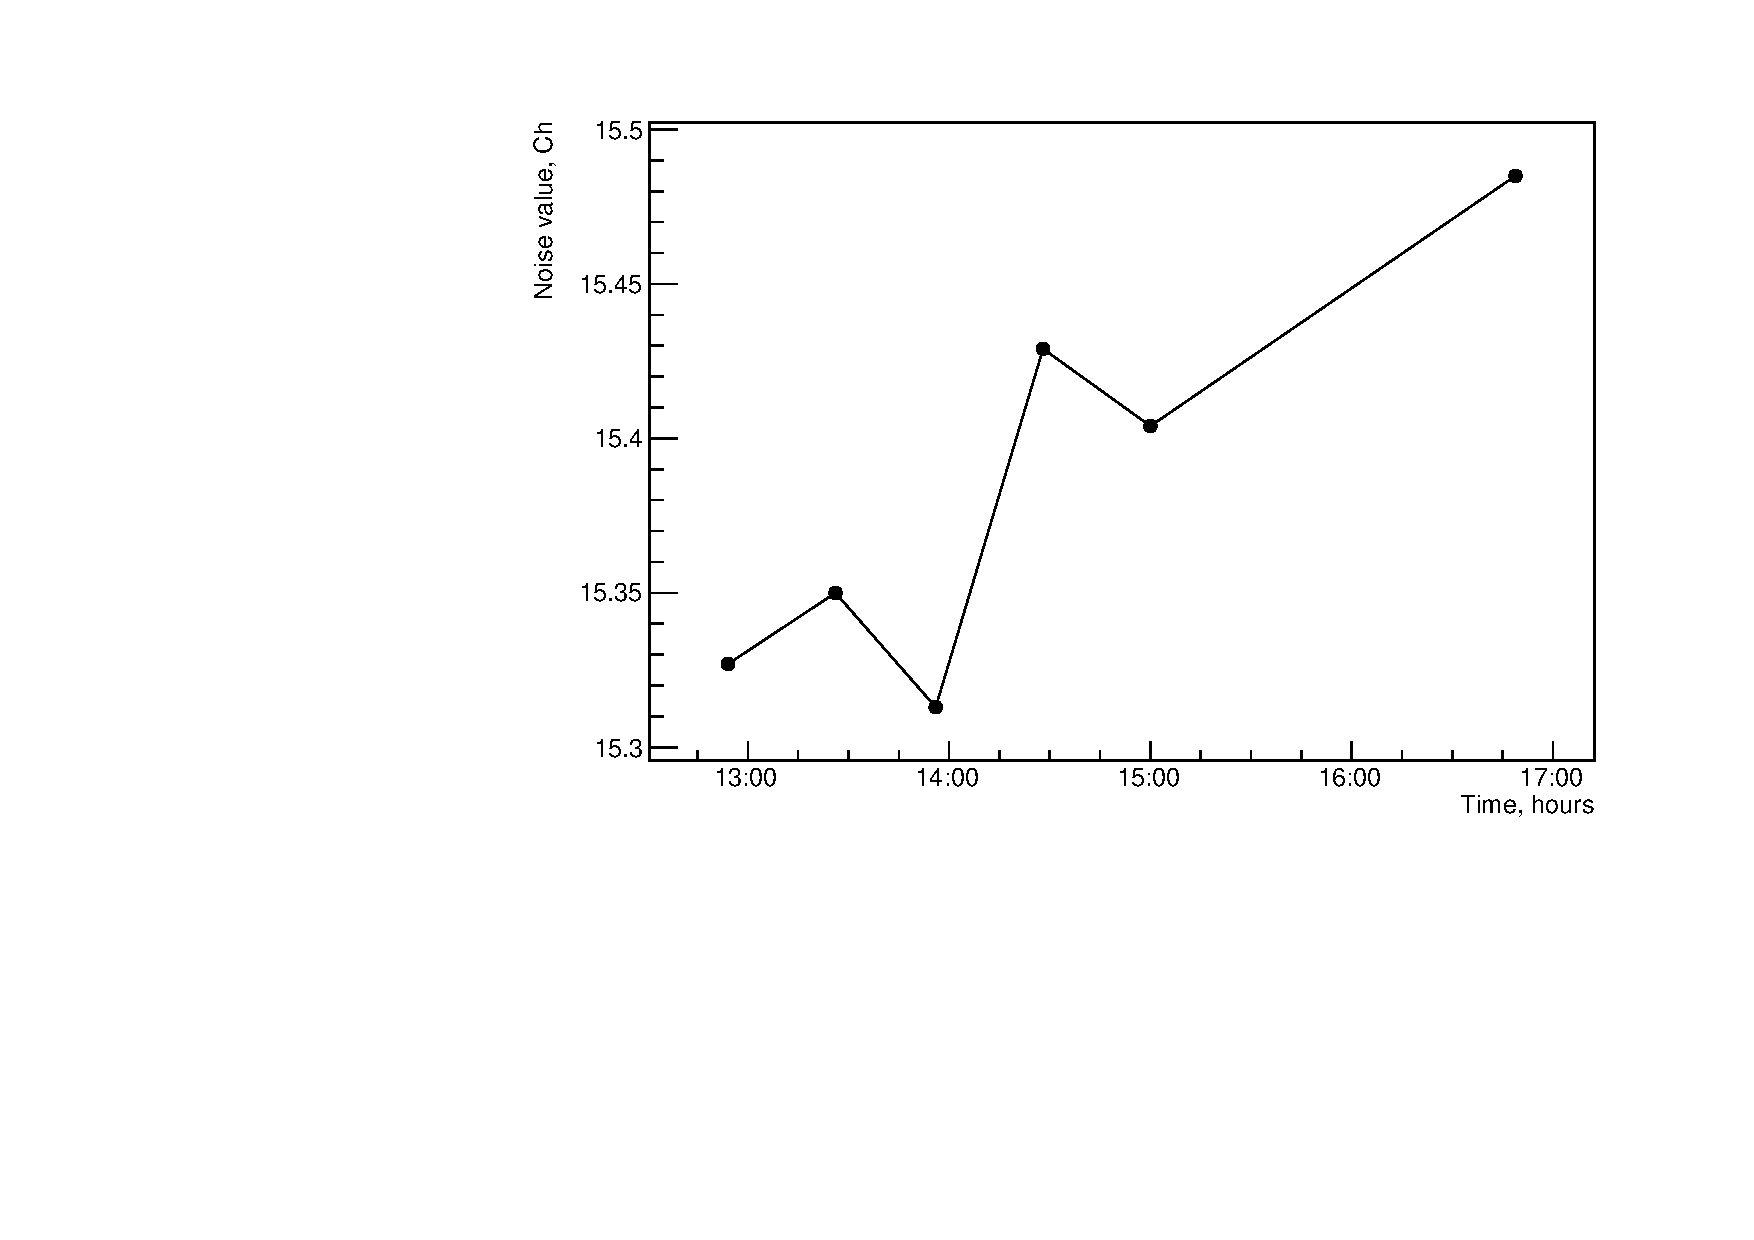
\includegraphics[width=1\linewidth]{img/Noise_time_drift.pdf}
		\caption{Уровень шумов}
	\end{subfigure}%
	\begin{subfigure}{.5\textwidth}
		\centering
		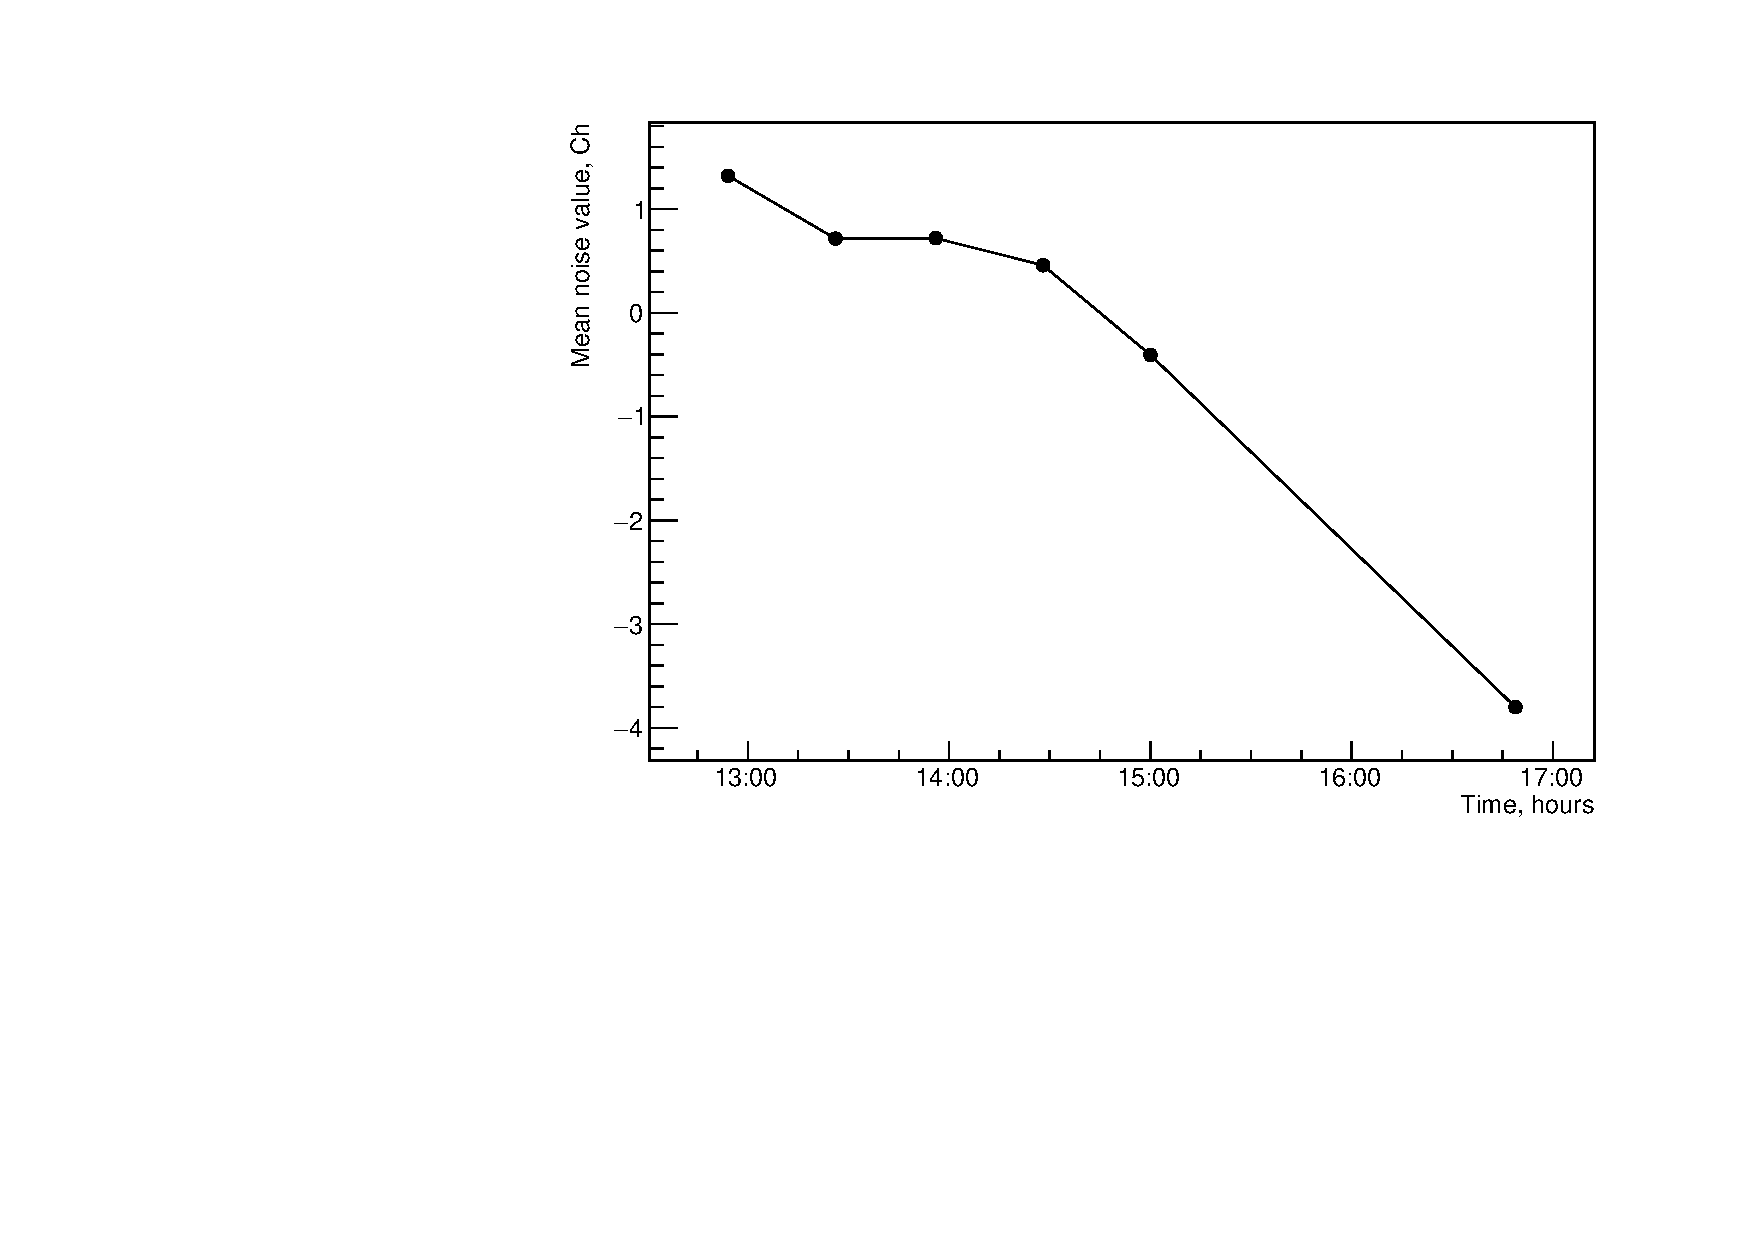
\includegraphics[width=1\linewidth]{img/Mean_time_drift.pdf}
		\caption{Среднее значение шума}
	\end{subfigure}
	\caption{Временной дрейф параметров шумовых событий: уровня шума и среднего значения шума. Каждая точка - среднее по $3\cdot10^7$ значений. В обоих случаях наблюдается линейный тренд. Статистические ошибки в точках малы и на графиках не видны}
	\label{fig:Noise_gr}
\end{figure}
Относительное изменение уровня шума за 4 часа составило $0.01~\sigma$, а дрейф среднего значения -- $0.33~\sigma$. Установившееся значение уровня шумов скорее всего зависит от температурного дрейфа электроники. Это является отдельной довольно обширной темой и в данной работе рассматриваться не будет. Однако, необходимы дополнительные долговременные эксперименты, которые смогут показать, каков максимально достижимый уровень шумов системы и насколько сдвигаются нулевые значения АЦП. Тем не менее, промежуточные результаты показали, что для <<Лазерного поляриметра>> это не является критичным.  
\section{Определение коэффициента усиления}
\label{sec:ampl_с}
При исследовании новой модели детектора необходимо различными методами проверить правильность работы, как ускоряющей структуры, так и вычитывающей электроники. Это можно сделать путём измерения коэффициента усиления детектора. 
%Стоит отметить, что зарегистрировать ионизацию первичной частицы достаточно сложно ввиду малого количества заряда. Для этого необходимы высокочувствительные АЦП. Однако, при использовании 
Коэффициент усиления в данной работе определяется как отношение зарегистрированного считывающей структурой заряда кластера к количеству частиц первичной ионизации, образованных в индукционном промежутке. 
Количество частиц первичной ионизации найдем, используя средние ионизационные потери и количество энергии, необходимое для образования ион--электронной пары. Известно, что потери энергии электронов в тонких слоях описываются модифицированной формулой Бете-Блоха:
\begin{equation}
\cfrac{dE}{dx} = \cfrac{2\pi N_0 e^4 Z\rho}{m_e c^2 \beta^2 A}\biggl[ln \bigg(\cfrac{ m_ec^2T\beta^2\gamma^2}{2I^2}\bigg) + f_{corr}(\beta)\biggr],
\label{eq:Bethe_Bloch}
\end{equation}
где $N_0$ -- число Авогадро, $e$ -- элементарный электрический заряд, $m_e$ -- масса электрона, $c$ -- скорость света, $\beta = v/c$ -- отношение скорости частицы к скорости света, $Z$ -- зарядовое число, $A$ -- массовое число, $\rho$ -- плотность вещества, $T$ -- кинетическая энергия электронов, $I$ -- энергия образования ион--электронной пары, $f_{coor}(\beta)$ -- функция, которая содержит поправки в случае $\beta \sim 1$. Параметры $A,Z,\rho$ относятся к веществу--радиатору т.е. к газовой смеси, которой заполнен детектор.
\par Вычисление показало, что средние потери энергии электронов с энергией $2.2~\MeV$ составляют $2.5~\keV/$см. Энергия образования одной ион--электронной пары в аргоне есть $26\eV$. Размер дрейфового промежутка -- 3 мм. Количество первичных электронов:
\begin{equation}
	N_e = \frac{dE/dx~\Delta x}{W} =\frac {2400~\eV/cm \cdot 0.3~cm}{26~\eV} = 28
\end{equation}
Зная средний заряд кластера $\langle Q\rangle$, можно определить коэффициент усиления системы GEM: 
\begin{equation}
K = \frac{\langle Q\rangle}{\langle N_e \rangle\ W},
\label{eq:ampl_k}
\end{equation}
где $I = 26~\eV$ -- средняя энергия образования ион-электронной пары в аргоне. 
\par Такой метод определения коэффициента усиления имеет один недостаток: в эксперименте определить средний заряд кластера достаточно трудно т.к. существуют ограничения электроники на максимальное измеренное значение. Более того, средний заряд кластера имеет распределение Ландау, параметром которого является наиболее вероятный заряд кластера. Поэтому вместо средних ионизационных потерь необходимо рассчитывать наиболее вероятные. Выражение для них можно записать следующим образом:
\begin{equation}
\Delta_p = \xi\biggl[ln \bigg(\cfrac{ m_ec^2T\beta^2\gamma^2}{2I^2}\bigg) + ln\bigg(\frac{\xi}{I}\bigg) + j - \beta^2 \biggr],
\label{eq:MP_energy_loss}
\end{equation}
где $j=0.2$, а параметр $\xi$ задается формулой:
\begin{equation}
\xi = 2\pi r_0^2 N_A m_ec^2\frac{Z}{A} \frac{\rho x} {\beta^2}, 
\end{equation}
где $r_0$ -- классический радиус электрона, $N_A$ -- число Авогадро. Оценка наиболее вероятных потерь в дрейфовом промежутке дает значение  $\Delta_p = 685~\eV$, а наиболее вероятное количество электронов $[N_e] = 26$, что на самом деле довольно близко к среднему значению.
%https://arxiv.org/pdf/1110.6761.pdf 
\subsection{Постановка эксперимента}
Для определения коэффициента усиления детектор облучался $2.2~\MeV$ электронами источника $Sr-90$, который располагался на герметичном кожухе детектора. Т.к. энергии электронов не хватало, чтобы пройти сквозь детектор, организация внешнего триггера по схеме совпадений не представлялась возможной. Поэтому запуск детектора проводился в автоматическом режиме.
\begin{figure}[H]
	\centering
	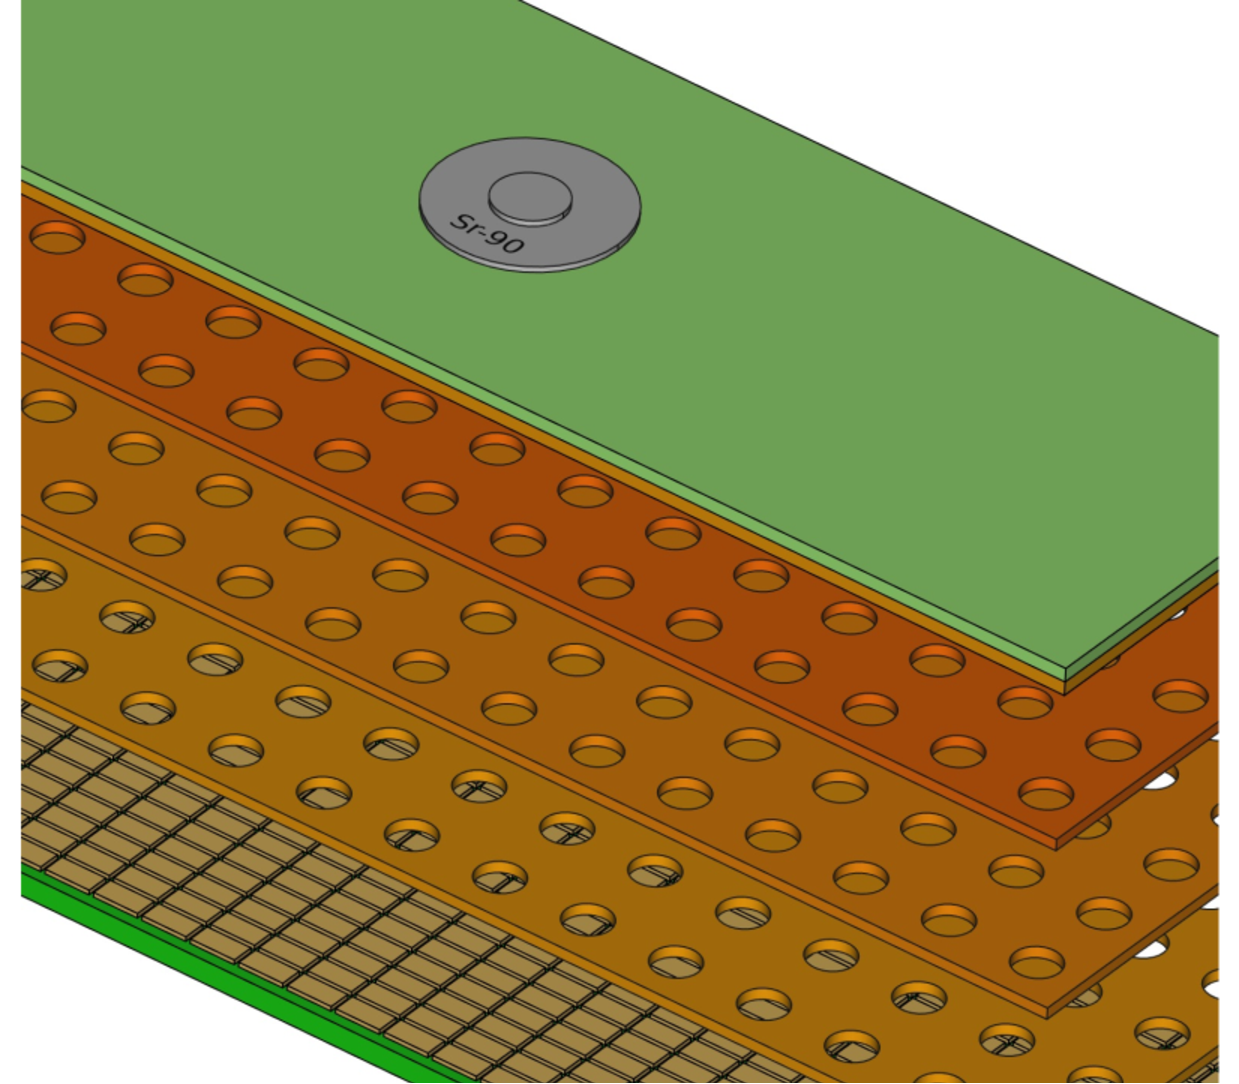
\includegraphics[height = 4 cm, width= 5.8cm]{img/GEM_Sr_source.pdf}
	\caption{Расположение источника относительно ускоряющей структуры}
	\label{fig:det_scheme+sr90}
\end{figure}
Электроны из источника проникали в газовый объем детектора и теряли энергию посредством ионизации. 
Первичная ионизация из дрейфового промежутка попадала в ускоряющую структуру, где происходило образование электронных лавин. Затем они проходили через два транспортных промежутка между GEM--электродами и попадали в индукционный промежуток. Заряд электронных лавин регистрировался считывающей структурой. По рассчитанному выше значению первичной ионизации и среднему заряду кластера определялся коэффициент усиления детектора. Цель эксперимента: проверить зависимость коэффициента усиления от напряжения. Для корректно работающей усиливающей и считывающей систем данная зависимость должна быть иметь экспоненциальный рост с увеличением напряжения. Набор статистики проходил в 7 точках по напряжению на ускоряющей структуре: от 3100 до 3450 В.

\subsection{Обработка и анализ полученных данных}
Полученные сырые данные обрабатывались с использованием алгоритмов, описанных в пункте \ref{sec:event_analysis}. После этого для каждого набора событий были построены распределения по заряду в кластерах. Для нахождения наиболее вероятного значения заряда экспериментальные гистограммы подгонялись функцией Ландау. После перевода каналов АЦП в единицы заряда коэффициент усиления находился по формуле \ref{eq:ampl_k}. На Рис. \ref{fig:charge_landau} можно видеть распределения по заряду кластера для двух точек по напряжению. 
\begin{figure}[h]
\centering
\begin{subfigure}{.45\textwidth}
	\centering
	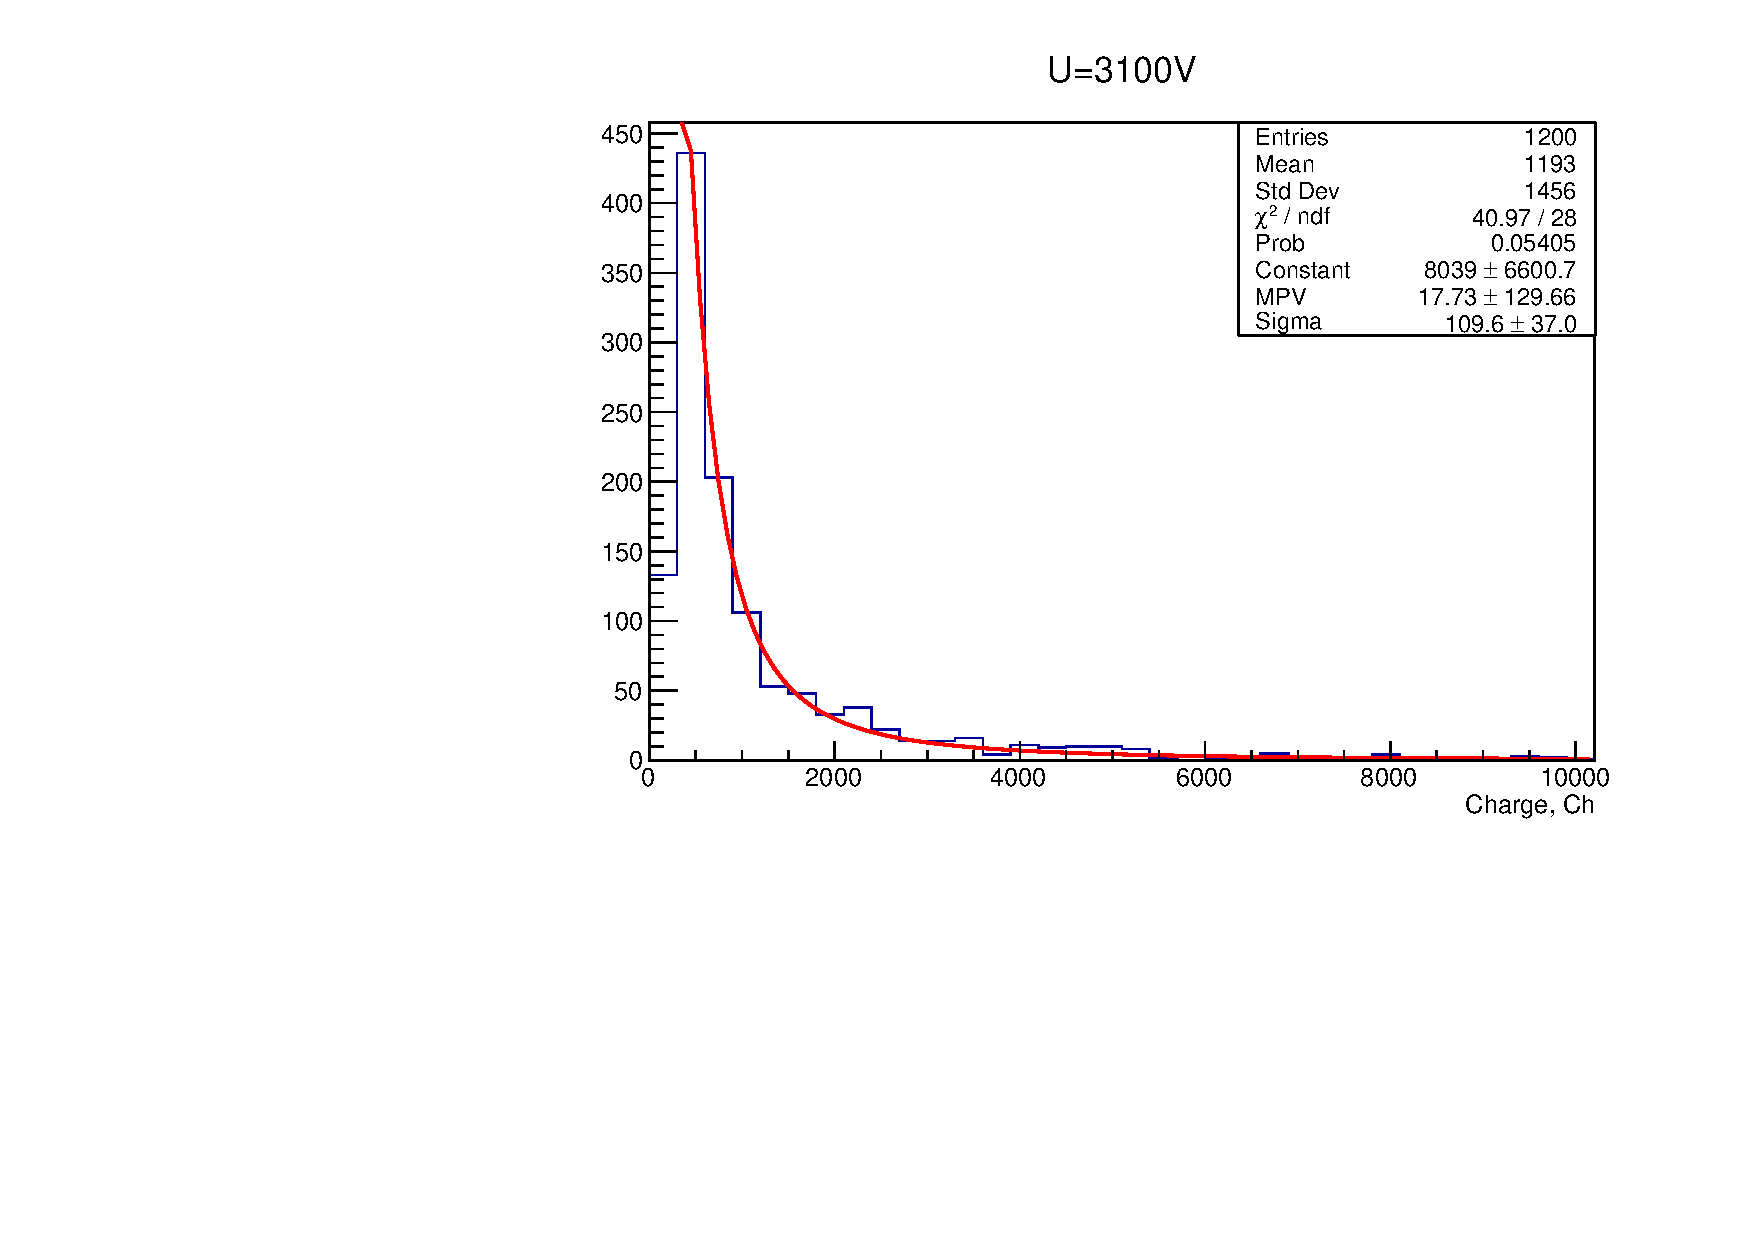
\includegraphics[width=1\linewidth]{img/3100.pdf}
	\caption{Напряжение на ускоряющей структуре 3100 В}
\end{subfigure}%
\hspace{20pt}
\begin{subfigure}{.45\textwidth}
	\centering
	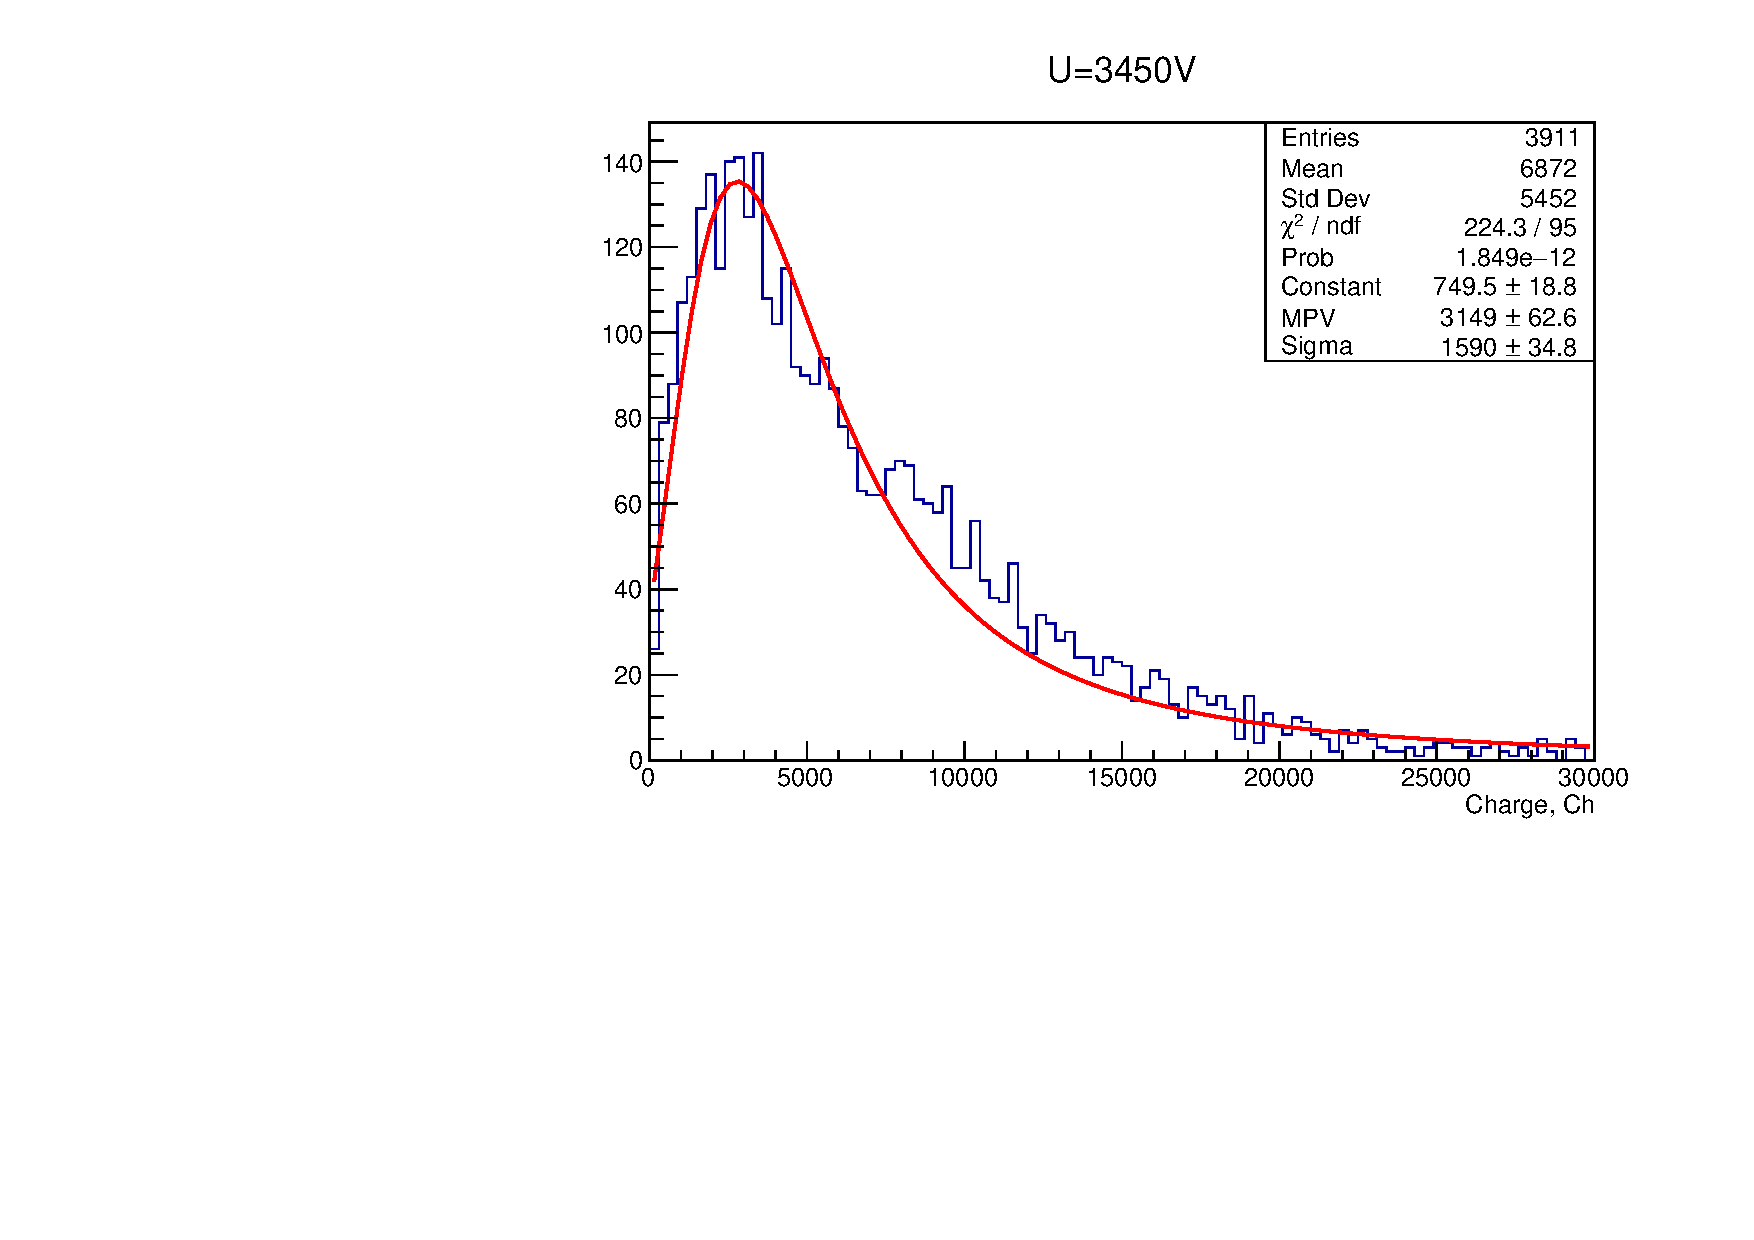
\includegraphics[width=1\linewidth]{img/3450.pdf}
	\caption{Напряжение на ускоряющей структуре 3450 В}
\end{subfigure}
\caption{Распределения по заряду кластера для разных значений напряжений на ускоряющей структуры детектора. Для напряжения 3100 В эффективность разделения сигнал--шум мала, поэтому положение пика распределения точно определить не получилось.}
\label{fig:charge_landau}
\end{figure}

\subsection{Результаты}
На Рис. \ref{fig:ampl_graph} представлены результаты измерений коэффициента усиления детектора. Для точек, где достоверно определен пик распределения Ландау наблюдается экспоненциальный тренд. Это указывает на правильную работу систем детектора.
\begin{figure}[h]
	\centering
	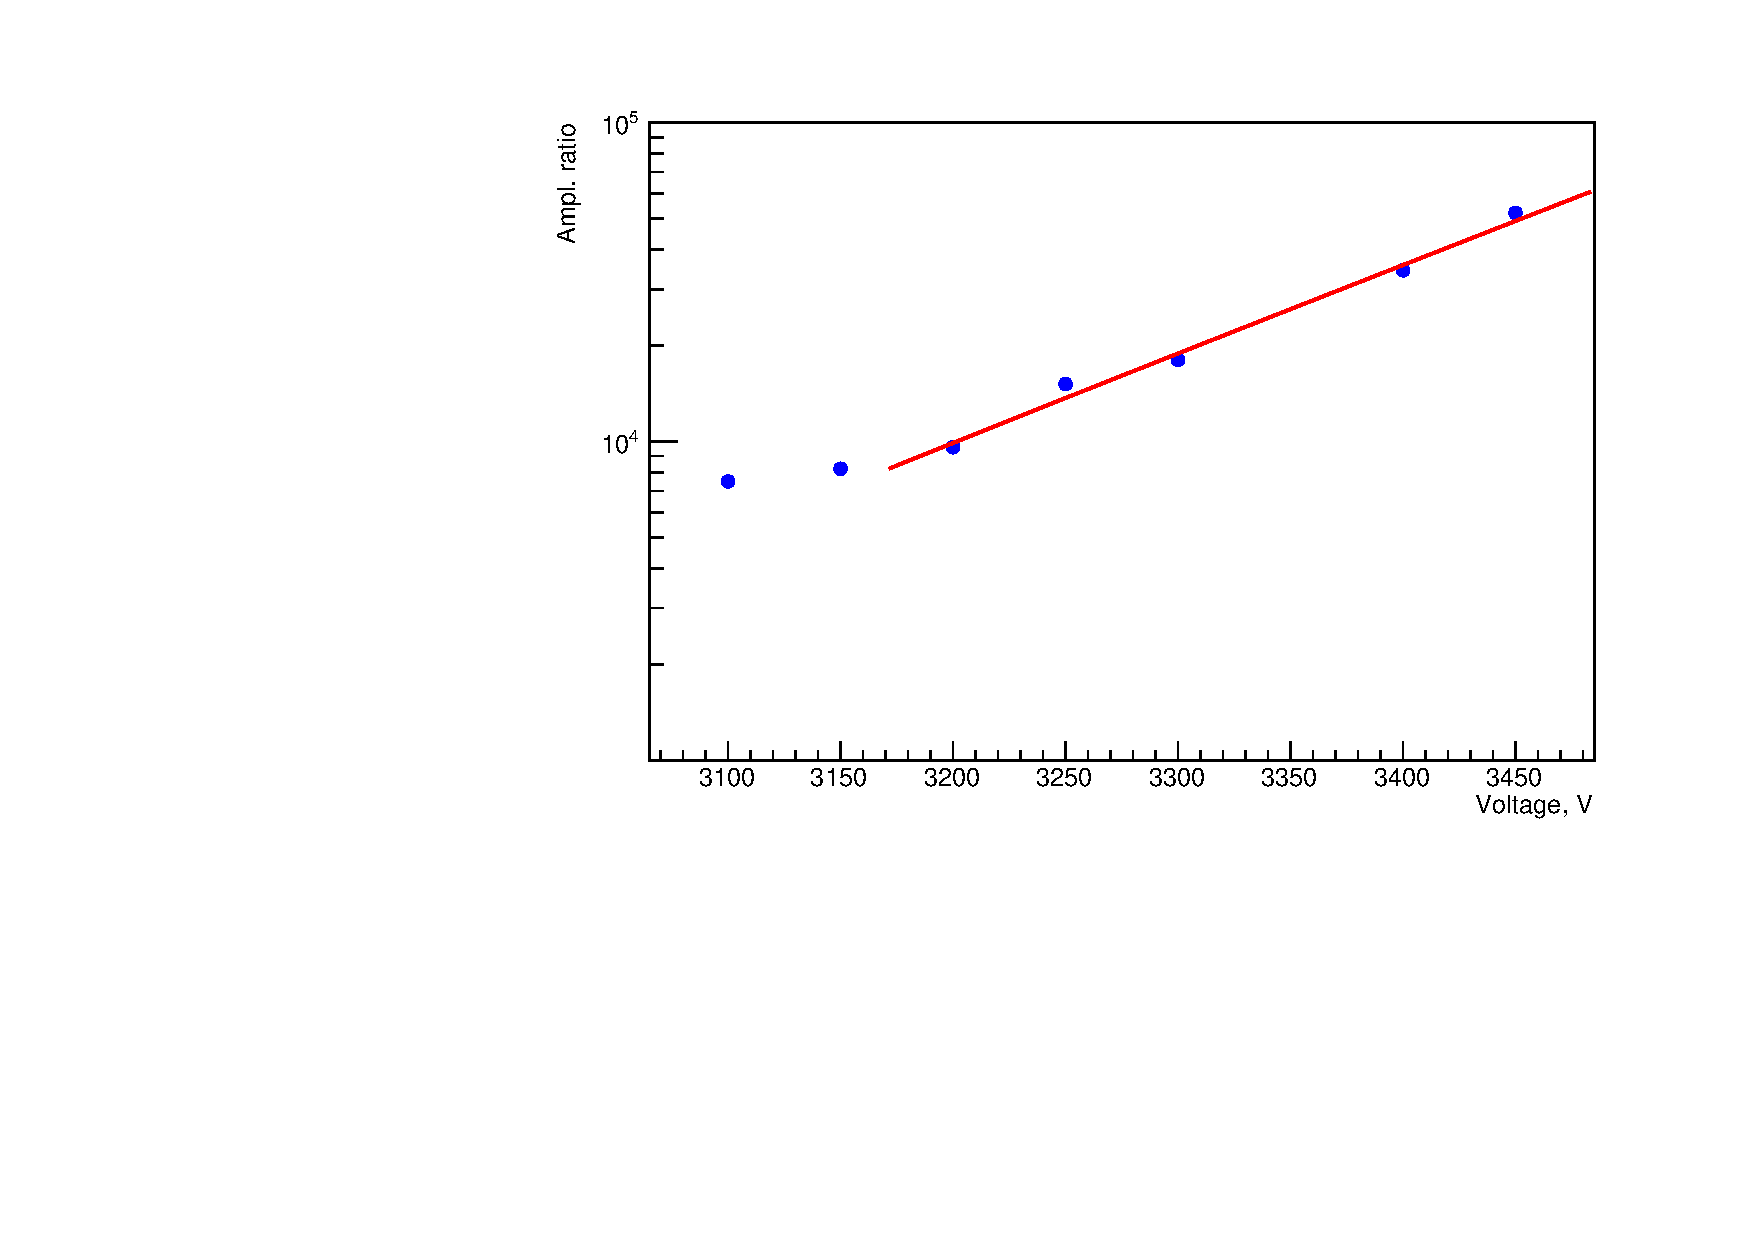
\includegraphics[width = 10cm]{img/Ampl_gr_log.pdf}
	\caption{Зависимость коэффициента усиления детектора от напряжения на ускоряющей структуре. Красная линия соответствует подгонке экспонентой.}
	\label{fig:ampl_graph}
\end{figure}
Максимальный коэффициент усиления, достигнутый при напряжении GEM--электродах 4500 В, составляет примерно 58000. Так же, при значении коэффициента усиления меньше 10000 достоверность разделения сигнала и шума резко уменьшается, что видно по количеству событий, отмеченных программой как сигнальные: при напряжении 3100 В было обработано 1200 сигнальных событий против 3900 при напряжении 3450 В. В точках с напряжением 3100 и 3150 В пик распределения Ландау был под границей шумов, поэтому его положение определялось лишь по правому склону распределения. Этим вызвана ошибка определения среднего заряда кластера, что привело к выполаживанию графика коэффициента усиления.

\section{Определение эффективности регистрации}
Еще одним параметром, который является ключевым для детектора, работающего в установке <<Лазерный поляриметр>>, является эффективность регистрации -- отношение числа зарегистрированных событий к их полному числу. Рассмотрим классическую схему для определения эффективности регистрации детекторов, которая подробно описана например в \cite{grupen}. Пусть имеется три детектора: D1, D2 и D3 с эффективностями $\varepsilon_1, \varepsilon_2$ и $\varepsilon_3$ соответственно. Требуется найти эффективность регистрации одного из них (для определенности выберем D1). Всего частиц, регистрируемых детекторами, $N_0$. Детекторы D2 и D3 необходимо включить в схему совпадений,т.е. сигнал о зарегистрированной частице должен генерироваться только тогда, когда они сработали одновременно. Это необходимо для эффективной фильтрации шумовых срабатываний. Схема из двух детекторов сможет зарегистрировать лишь $N_{23}$ событий. В предположении того, что акты регистрации частицы в двух детекторах абсолютно независимы, можно выразить $N_{23}$ как: 
\begin{equation}
N_{23} = \varepsilon_2\varepsilon_3 N_0.
\end{equation}
Если теперь добавить к этой схеме третий детектор и подсчитывать события, которые дали сигнал одновременно в трех детекторах, то их число будет: 
\begin{equation}
N_{123} = \varepsilon_1\varepsilon_2 \varepsilon_3 N_0.
\end{equation}
Отсюда можно определить эффективность регистрации третьего детектора: 
\begin{equation}
\varepsilon_1 = \frac{N_{123}}{N_{23}}
\end{equation}
Таким образом, для определения $\varepsilon_1$ необходимо знать количества событий, регистрируемых двумя схемами совпадений, одна из которых включает два детектора, а другая -- все три. Данный метод является простым и надежным, но не учитывает геометрических параметров детекторов, что так же может сильно повлиять на определяемое значение $\varepsilon$.
\subsection{Постановка эксперимента}
Измерение эффективности регистрации детектора <<Лазерного поляриметра>> было проведено на выведенном пучке электронов ускорителя ВЭПП-4М. Сначала был получен пучок тормозных гамма--квантов, которые затем конвертировались на свинцовой мишени в электрон--позитронные пары. Затем происходил отбор электронов по энергии с помощью спектрометрического магнита, за которым располагались детектирующая система.
 \begin{figure}[h]
 	\centering
 	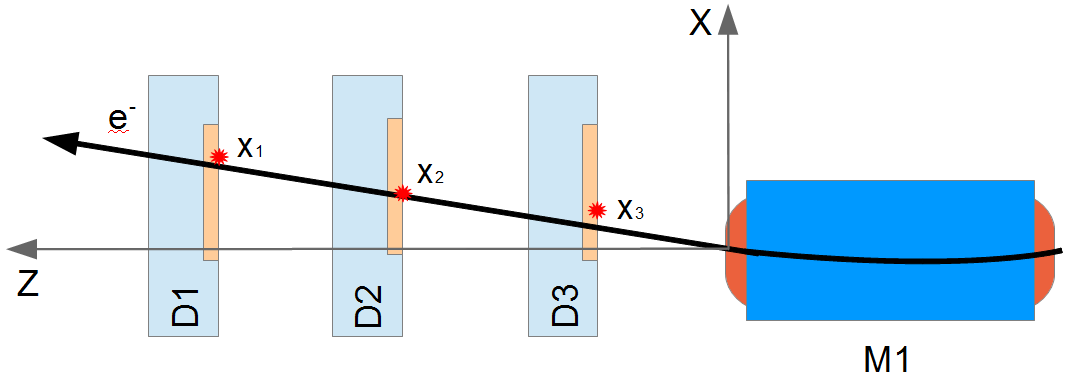
\includegraphics[width= 12cm]{img/reg_eff_exp_scheme.png}
 	\caption{Принципиальная схема установки для определения эффективности регистрации и пространственного разрешения на выведенном пучке ускорителя ВЭПП-4М. М1 -- спектрометрический магнит, D2,D3 -- вспомогательные детекторы, D1 -- исследуемый детектор.}
 	\label{fig:test_beam_scheme}
 \end{figure}
Для реализации схем совпадений помимо исследуемого детектора были использованы ещё два, которые работают в составе установки <<ДЕЙТОН>>. Это двухкоординатные GEM--детекторы с размером чувствительной области $160 \times 40$\,мм, применяемые на установке <<ДЕЙТОН>>. Все элементы схемы были позиционированы с помощью лазерных уровней и подключены к системе сбора данных выведенного пучка для того, чтобы получать сигналы триггера, который расположен сразу после мишени--конвертера. В ходе эксперимента тремя детекторами регистрировались координаты электронов выведенного пучка. Измерения проводились, начиная с напряжения на ускоряющей структуре 3200 В в шести точках с шагом 50 В. При последующей работе с данными события из разных детекторов связывались с помощью их порядкового номера в файлах. Стоит отметить, что данные, полученные при работе на выведенном пучке, были так же использованы для определения пространственного разрешения детектора. 

\subsection{Обработка и анализ результатов эксперимента}
Для удобства последующей работы на основе сырых данных были созданы деревья (ROOT TTree), которые содержали три ветви: две координаты и номер события. Для определения координат зарегистрированных частиц был программно реализован метод нахождения центра тяжести кластера. Его суть заключается в следующем: сначала определяются каналы, сигнал в которых превышает шумовой, затем по горизонтальной и вертикальной координате производится независимое суммирование вида: 
\begin{equation}
 \langle x \rangle = \frac{\sum_{i}q_i x_i}{\sum_{i}q_i},
\end{equation}
где $q_i$ -- заряд канала с координатой $x_i$. Нормировка производилось на полный заряд кластера.
\par По причине того, что чувствительная область детектора для поляриметра не охватывала весь пучок, стандартный алгоритм вычисления эффективности регистрации был модифицирован: в него добавлен учет геометрических параметров детектора и их влияние на конечную величину эффективности. Ниже приведена последовательность операций с данными для данного алгоритма.
\begin{itemize}
	\item Сначала отбирались события, попавшие в центральную область детектора <<Лазерного поляриметра>>
	\item Затем для этой выборки находились средние значения координат и дисперсии в дополнительных детекторах D2 и D3. 
	\item В детекторах D2 и D3 выделялись области с центром в точках, соответствующих средним значениям по выборке и размером в одно стандартное отклонение. 
	\item После этого \textit {по всему набору} подсчитывались события, которые попадают в выделенные области (в том числе и незарегистрированные исследуемым детектором.)
	\item Отношение числа событий из центральной области детектора <<Лазерного поляриметра>> к числу событий из выделенных областей дополнительных детекторов  регистрации. 
\end{itemize}

\subsection{Результаты}

\begin{figure}[h]
	\centering
	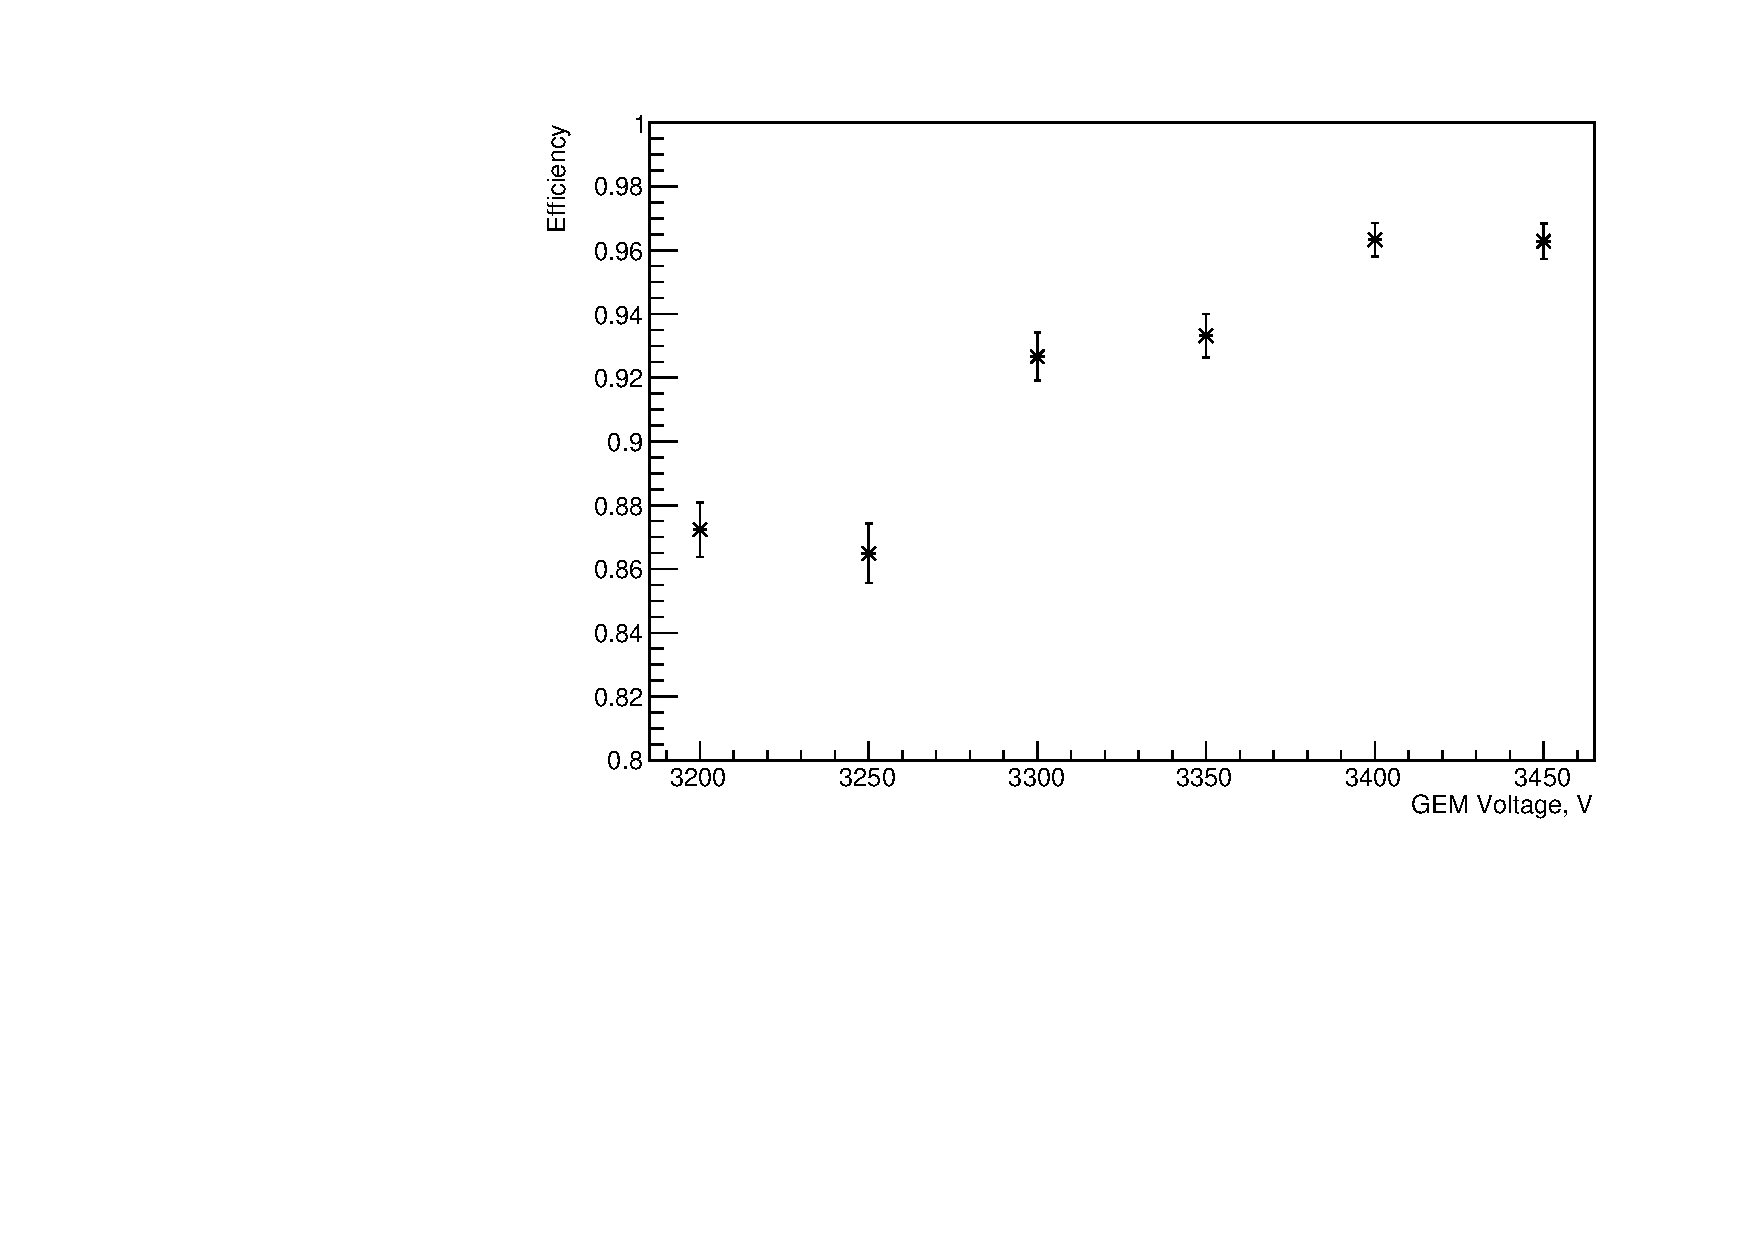
\includegraphics[width= 12cm]{img/eff_plot.pdf}
	\caption{Зависимость эффективности регистрации от напряжения на ускоряющей структуре.}
	\label{fig:eff_gr}
\end{figure}

\section{Определение пространственного разрешения}
\endgroup
\newpage
\chapter*{Заключение}
В ходе работы исследовался прототип координатного детектора фотонов, который планируется использовать в составе системы измерения энергии пучков ускорителя ВЭПП-4М. Сначала был изучены теоретические основы метода измерения энергии по резонансной деполяризации частиц в ускорителе. На основе полученных знаний сформированы требования к координатному детектору, а также  пояснена мотивация применения именно микроструктурных детекторов в конкретном случае. 
\par Далее была описана конструкция прототипа детектора, его технические характеристики. После этого рассмотрены особенности сбора и обработки данных для извлечения из них информации о координатах ионизирующих частиц. На языке Python написана библиотека в которой реализовано чтение файлов сырых данных с детектора, вычитание пьедесталов, нахождение кластеров, определение координат кластера методом центра тяжести и другие функции. 
\par В финальной части работы исследовались характеристики детектора. Определен уровень шумов, значение которого составило около $6000 e^-$. Данная информация необходима для правильного выбора порогового уровня при разделении сигнала и шума. С помощью радиоактивного изотопа проведено исследование зависимости коэффициента усиления от напряжения на ускоряющей структуре. Экспериментальные данные подчиняются экспоненциальному тренду, что говорит о правильной работе ускоряющей структуры и считывающей электроники. 
\par На выведенном пучке ускорителя ВЭПП-4М были измерены эффективность регистрации и пространственное разрешение. Максимально достигнутое значение эффективности при напряжении на ускоряющей структуре 3450 В составило $96 \pm 1\%$. Пространственное разрешение измерено отдельно для каждой из координат: для вертикальной координаты $\sigma_y = 0.258\pm0.007\pm0.017$\,мм, для горизонтальной $\sigma_x = 0.44\pm0.01$\,мм. Эти значения меньше, чем теоретическое предсказание для считывающей схемы, работающей в режиме идентификации треков. Объясняется это успешным применением метода центра тяжести при нахождении координат частиц, которые вызвали срабатывание группы каналов. 
\par Таким образом, первые исследования характеристик детектора для установки <<Лазерный поляриметр>> показали, что его можно успешно применять в системе измерения энергии. 
\newpage
%\section{Предел Рейтера и его зависимость от электрического поля в индукционном промежутке}
\label{sec:raether_exp}
Существенным параметром для детекторов, построенных с использованием ГЭУ, является коэффициент усиления. Существует два основных пути достижения его требуемых значений: 
\begin{itemize}
	\item обеспечение высокой электрической прочности электрода ГЭУ и приложение к нему более высоких напряжений
	\item использование несколько последовательно расположенных ГЭУ
\end{itemize}
Каждый из них имеет свои ограничения на применимость. ТУТ ОПИСАТЬ ПРО ПЕРВЫЙ МЕТОД.\par
Последовательное расположение нескольких ГЭУ с одной стороны вызывает усложнение конструкции детектора и увеличение количества материала на пути частицы. С другой стороны, напряжение на каждом электроде будет существенно ниже, чем в случае с одним ГЭУ. Нами было выдвинуто предположение
%\newpage
\addcontentsline{toc}{chapter}{Список литературы}  
\bibliographystyle{include/utf8gost705u}
\renewcommand\bibname{Список литературы}
\bibliography{bibliography.bib}
\end{document}